\documentclass[12pt,openright,oneside,a4paper,brazil]{abntex2}

% --- Codificação e Idioma ---
\usepackage[utf8]{inputenc}
\usepackage[T1]{fontenc}
\usepackage{lmodern}
\usepackage{indentfirst}

% --- Geometria da Página (Padrão ABNT / UFMG) ---
\usepackage[top=30mm,bottom=20mm,left=30mm,right=20mm]{geometry}

% --- Matemática e Tipografia Avançada ---
\usepackage{amsmath,amsfonts,amssymb}
\usepackage{microtype}
\usepackage{booktabs}
\usepackage{multirow}
\usepackage{siunitx}
\usepackage{adjustbox}

% --- Controle de Posição de Flutuantes ---
\usepackage{flafter}

% --- Figuras e Gráficos ---
\usepackage{graphicx}
\graphicspath{{figuras/}}

% --- Links e Cores ---
\usepackage{xcolor}
\definecolor{primaryblue}{RGB}{18, 64, 118}
\definecolor{darkred}{RGB}{140, 20, 20}
\hypersetup{
    colorlinks=true,
    linkcolor=primaryblue,
    citecolor=primaryblue,
    urlcolor=primaryblue
}

% --- Referências Inteligentes e Citações ABNT ---
\usepackage[brazilian, capitalise, noabbrev, nameinlink]{cleveref}
\usepackage[alf]{abntex2cite} 
 
% --- Metadados do Trabalho Acadêmico (abntex2) ---
\instituicao{%
  UNIVERSIDADE FEDERAL DE MINAS GERAIS \par
  ESCOLA DE ENGENHARIA \par
  PROGRAMA DE PÓS-GRADUAÇÃO EM ENGENHARIA ELÉTRICA
}
\titulo{Consolidação Experimental e Proposta de Modelagem Computacional de Circuitos Hipocampais}
\autor{Wagner Mathias Fonseca Franklin}
\local{Belo Horizonte}
\data{2026}
\orientador{Prof. Dr. Márcio Flávio Dutra Moraes}
\coorientador{Prof. Dr. Hani Camille Yehia}
\tipotrabalho{Relatório de Qualificação de Mestrado}
\preambulo{Relatório de consolidação de dados coletados em experimentos \textit{in vivo} e de modelagem biofísica de microcircuitos hipocampais.} 

\makeatletter
\renewcommand{\folhaderostocontent}{
  \begin{center}
    {\ABNTEXchapterfont\large\imprimirinstituicao}
	
    \vspace*{\fill}\vspace*{\fill}
    \begin{center}
      \ABNTEXchapterfont\bfseries\Large\imprimirtitulo
    \end{center}
    \vspace*{\fill}
	
    \abntex@ifnotempty{\imprimirpreambulo}{%
      \hspace{.45\textwidth}
      \begin{minipage}{.5\textwidth}
      	\SingleSpacing
         \imprimirpreambulo
       \end{minipage}%
       \vspace*{\fill}
    }%

    {\ABNTEXchapterfont\large\imprimirautor\vspace*{\fill}}

    {\large\imprimirorientadorRotulo~\imprimirorientador\par}
    \abntex@ifnotempty{\imprimircoorientador}{%
       {\large\imprimircoorientadorRotulo~\imprimircoorientador}%
    }%
    \vspace*{\fill}

    {\large\imprimirlocal}
    \par
    {\large\imprimirdata}
    \vspace*{1cm}

  \end{center}
}
\makeatother

\begin{document}

% --- Elementos Pré-Textuais ---
% \pretextual

% \imprimircapa 
\imprimirfolhaderosto

% --- Resumo Objetivo ---
\setlength{\absparsep}{18pt}
\begin{resumo}
    Este trabalho consolida os resultados empíricos de microestimulação elétrica hipocampal em modelos animais de memória contextual e estabelece uma estrutura rigorosa de modelagem biofísica computacional em \textsf{Brian~2} para investigar o processamento temporal de sinais na sub-região CA3. Inicialmente, a análise metrológica dos testes comportamentais de preferência por objetos e rastreamento cinemático (\textit{pose estimation} via Behavython/DeepLabCut) revelou fontes críticas de viés físico intrínseco aos pares de objetos de vidro, além de subdimensionamento amostral que comprometeu o poder estatístico nos ensaios preliminares in vivo, delimitando com transparência o encerramento da fase cirúrgica em animais. Em seguida, formulou-se um modelo biofísico de microcircuito contendo neurônios piramidais excitatórios de adaptação lenta (\textit{Regular Spiking}) e interneurônios inibitórios rápidos perissomáticos $\text{PV}^+$ (\textit{Fast Spiking}) com dinâmica de Izhikevich, acoplados a plasticidade sináptica de curto prazo de Tsodyks-Markram ($\tau_{\text{rec}} = \qty{600}{\milli\second}$) e condutâncias de \textit{shunting}. No Experimento~1 (estimulação elétrica contínua), demonstrou-se que a estimulação em malha aberta induz colapso vesicular acentuado ($R_{\text{ss}} \approx 0{,}11$, atenuação de $89\%$ no feedback excitatório) e inibição perissomática rápida. Sob a ótica de taxa de disparo escalar, o Teste de Equivalência Biológica (TOST, margem de $15\%$) comprovou equivalência estatística estrita entre os padrões ($p_{\text{TOST}} = 7{,}12 \times 10^{-7}$, $p < 0{,}001$), enquanto no domínio temporal a correlação linear de Pearson no Histograma Temporal Peri-Estímulo (PSTH por bins de $\qty{14}{\milli\second}$) revelou desfasamento estrito ($r = -0{,}3035$). No Experimento~2 (transdução optogenética via ChR2 e Chronos com cinética fotoquímica calibrada), comprovou-se que embora a variante rápida Chronos feche entre pulsos adjacentes ($O_{\text{mín}} \approx 0$), a integral intracelular de cálcio $[\text{Ca}^{2+}](t)$ (indicador de c-Fos) é invariante à dose total de fótons pareada em malha aberta ($p = 0{,}2791$), justificando quantitativamente a ausência de diferença observada na histologia de bancada ($p = 0{,}9888$). Conclui-se que protocolos temporais em malha aberta requerem o recrutamento de não linearidades biofísicas adicionais, propondo-se como continuidade a investigação in silico de modulação por rajadas em alta frequência (\textit{bursting}), janelas de plasticidade dependente do tempo de disparo (STDP) e multiplexação óptica espectral no eixo CA3--CA1.

    \noindent \textbf{Palavras-chave}: Estimulação Elétrica. Neurociência Computacional. Microcircuitos Hipocampais. Modelo de Izhikevich. Dinâmica Sináptica de Tsodyks-Markram.
\end{resumo}

% --- Sumário (Índice de Capítulos) --- 
\pdfbookmark[0]{\contentsname}{toc}
\tableofcontents*
\cleardoublepage

% --- Elementos Textuais ---
\textual
\OnehalfSpacing

\chapter{Parâmetros Iniciais e Protocolo Institucional (CEUA)}

O protocolo experimental investigou se padrões temporais organizados de microestimulação elétrica ($\mu$ES) aplicados à região CA3 do hipocampo ventral são suficientes para codificar contextos artificiais associados a objetos físicos específicos, em um paradigma adaptado de reconhecimento de contexto-objeto \cite{dix1999}.

Todos os procedimentos foram estruturados em conformidade com as diretrizes do Conselho Nacional de Controle de Experimentação Animal (CONCEA) e com aprovação da Comissão de Ética no Uso de Animais da Universidade Federal de Minas Gerais (CEUA/UFMG). O protocolo original previu o emprego de camundongos C57BL/6 adultos machos, mantidos em biotério sob ciclo claro/escuro de 12 horas, temperatura controlada ($\qty{22}{\degreeCelsius}$), com livre acesso a água e ração.

Os animais foram submetidos a cirurgia estereotáxica sob anestesia inalatória (isoflurano), recebendo analgesia preventiva e cuidados pós-operatórios para consolidação do implante craniano. Microeletrodos bipolares concêntricos foram direcionados às coordenadas de CA3 ventral, com matriz de parafusos de ancoragem e blindagem elétrica para evitar artefatos eletromiográficos e garantir acoplamento mecânico estável durante a movimentação livre na arena.

Como sintetizado na \cref{tab:protocolo_ceua}, os animais foram submetidos a dois padrões de estímulo discretizados em palavras binárias de 10 bits distribuídas dentro do período de uma oscilação teta hipocampal ($\qty{140}{\milli\second}$, $\qty{7.14}{\hertz}$). Ambos os padrões entregam pulsos ativos dentro da janela de $\qty{140}{\milli\second}$ com densidade temporal específica, variando estritamente os intervalos inter-pulso (IPIs). A estimulação foi administrada em regime contínuo ao longo de cada sessão de treinamento e teste.


\begin{table}[tbp]
    \centering
    \setlength{\tabcolsep}{5pt}
    \caption{Parâmetros do protocolo experimental e de microestimulação elétrica ($\mu$ES).}
    \label{tab:protocolo_ceua}
    \begin{adjustbox}{max width=0.95\textwidth}
        \begin{tabular}{lll}
            \toprule
            \textbf{Parâmetro}     & \textbf{Especificação}              & \textbf{Observações}                                                                                      \\
            \midrule
            Área de Interesse      & CA3 Hipocampo Ventral               & Coordenadas: AP: \qty{-3.30}{\milli\meter}; ML: $\pm\,\qty{2.50}{\milli\meter}$; DV: \qty{-4.00}{\milli\meter} \\
            Tipo de Onda           & Pulso Quadrado Bifásico             & -                                                                                                         \\
            Amplitude de Corrente  & \qty{25}{\micro\ampere}              & -                                                                                                         \\
            Largura de Pulso       & \qty{100}{\micro\second}             & -                                                                                                         \\
            Frequência Portadora   & \qty{7.14}{\hertz} (Ritmo Teta)      & Período fundamental $T_{\text{teta}} = \qty{140}{\milli\second}$                                           \\
            Discretização Temporal & Palavra binária de $10\text{ bits}$ & \qty{14}{\milli\second} por bin temporal                                                                  \\
            Padrão 1 ($S_1$)       & \texttt{1010101101}                 & 6 pulsos ativos por ciclo teta                                                                            \\
            Padrão 2 ($S_2$)       & \texttt{1110010111}                 & 7 pulsos ativos por ciclo teta                                                                            \\
            Regime de Aplicação    & Contínuo                            & Ininterrupto durante todos os treinamentos e testes                                                       \\
            \bottomrule
        \end{tabular}
    \end{adjustbox}
\end{table}

\chapter{Testes de Preferência por Objeto em Animais Naive}

A validade interna de tarefas comportamentais de reconhecimento de objetos repousa sobre a premissa de que a atratividade intrínseca dos estímulos seja neutra, de modo que a exploração assimétrica reflita memória e aprendizagem, e não viés perceptivo ou neofobia espontânea \cite{ennaceur1988, antunes2012}. Para selecionar um par isento de preferência basal, foram conduzidos testes de simetria utilizando quatro combinações de objetos tridimensionais em animais \emph{naive} (sem cirurgia prévia).


A caracterização física dos pares avaliados está sumarizada na \cref{tab:testes_preferencia}, e a disposição espacial dos pares na arena aberta é ilustrada na \cref{fig:objetos_preferencia}.

\begin{table}[tbp]
    \centering
    \small
    \setlength{\tabcolsep}{4pt}
    \caption{Caracterização dos testes de preferência de objetos em animais \emph{naive}. Os mesmos dez animais foram usados para fazer os quatro testes.}
    \label{tab:testes_preferencia}
    \begin{adjustbox}{max width=0.95\textwidth}
        \begin{tabular}{cccc}
            \toprule
            Teste & Objetos                                                     & Material          & $N$ \\
            \midrule
            1     & Prisma Circular | Prisma Pentagonal                         & Impresso 3D (PLA) & 10  \\
            2     & Garrafa com tampa vermelha | Garrafa com tampa branca       & Plástico (PET)    & 10  \\
            3     & Prisma Triangular | Prisma Quadrangular                     & Impresso 3D (PLA) & 10  \\
            4     & Garrafa cilíndrica roxa | Garrafa quadrangular transparente & Vidro             & 10  \\
            \bottomrule
        \end{tabular}
    \end{adjustbox}
\end{table}

\begin{figure}[!ht]
    \centering
    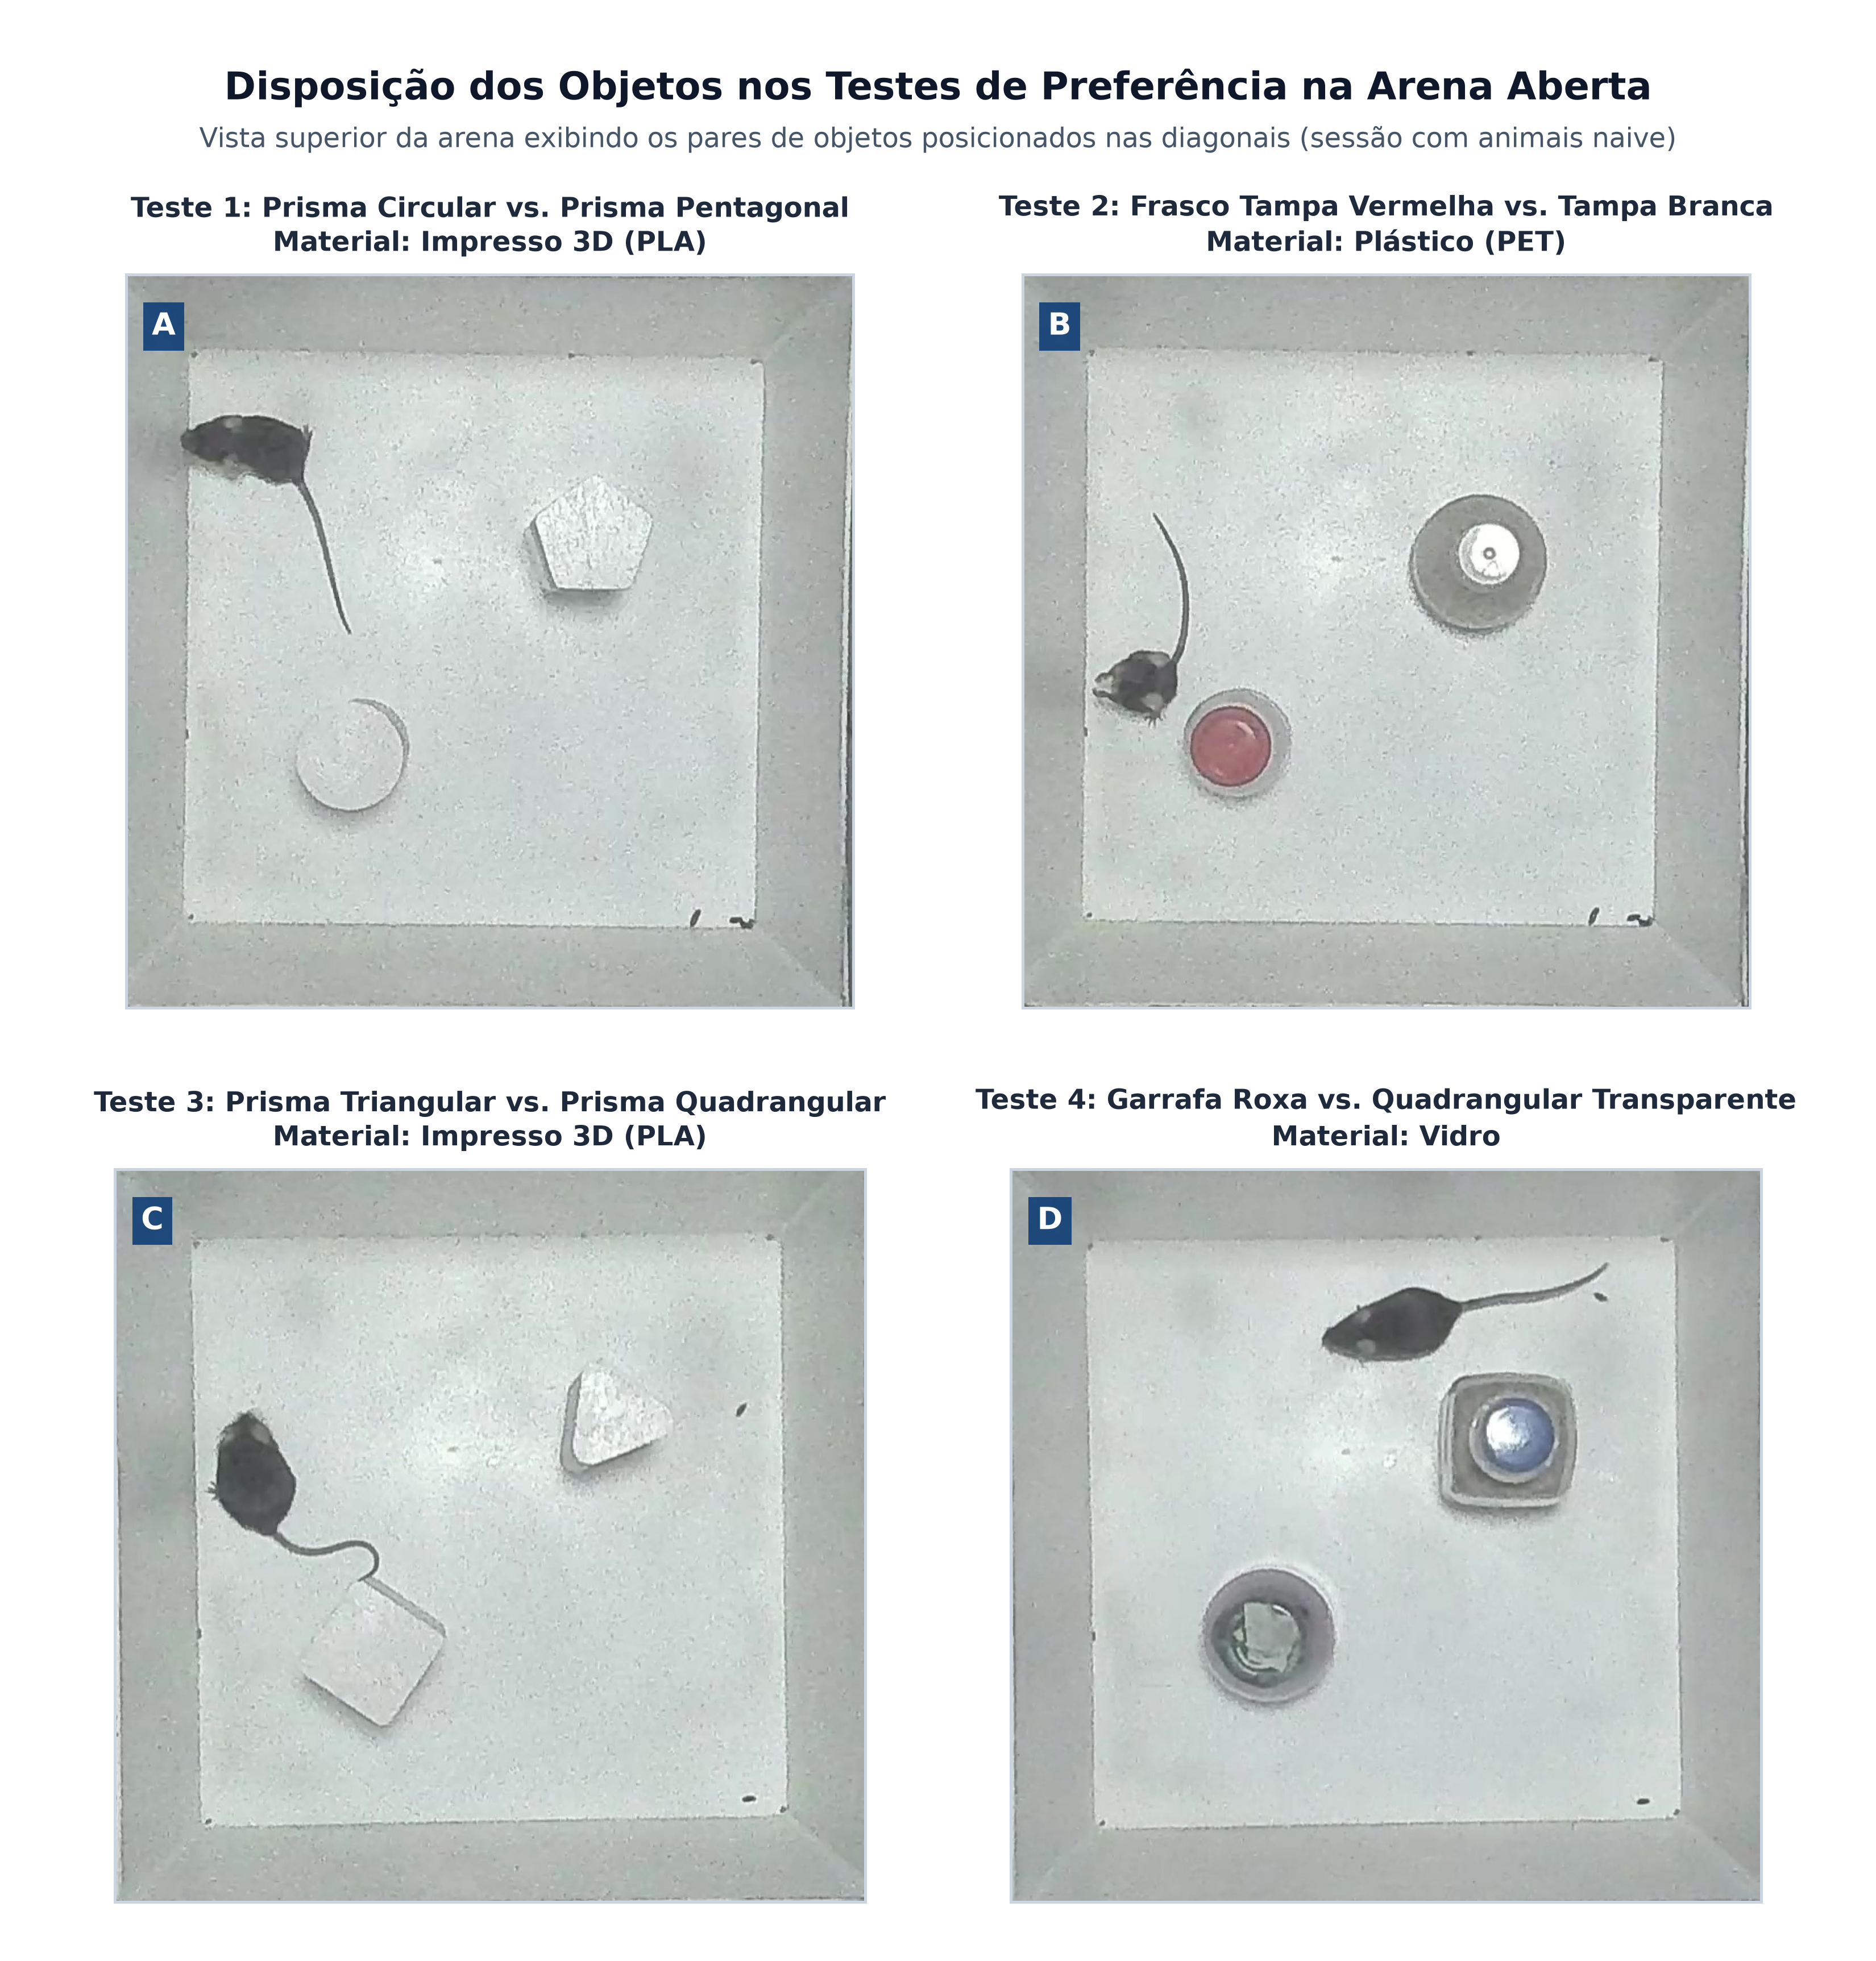
\includegraphics[width=0.9\textwidth]{painel_objetos_testes_preferencia.png}
    \caption{Disposição espacial dos pares de objetos posicionados nas diagonais da arena aberta durante os testes de preferência em animais \emph{naive}: (A) Teste~1 (Prisma Circular vs. Prisma Pentagonal em PLA); (B) Teste~2 (Frascos PET com tampa vermelha vs. tampa branca); (C) Teste~3 (Prisma Triangular vs. Prisma Quadrangular em PLA); (D) Teste~4 (Garrafa cilíndrica roxa vs. quadrangular transparente em vidro).}
    \label{fig:objetos_preferencia}
\end{figure}

O protocolo de aferição consistiu em cinco minutos de habituação prévia na arena vazia, seguida imediatamente pela introdução de dois objetos dispostos na diagonal, equidistantes das paredes e entre si, concedendo dez minutos para livre exploração dos roedores. Os tempos de interação focinho-objeto foram cronometrados e convertidos em proporções normalizadas de exploração.

Como evidenciado na \cref{fig:teste_preferencia}, os pares de objetos apresentaram perfis de atratividade marcadamente heterogêneos. Nos testes 1 e 2, não se identificou assimetria exploratória estatisticamente detectável. Contudo, enquanto o par 1 mostrou-se dispersivo, o par do Teste~2 (frascos PET) demonstrou neutralidade. Em contrapartida, os pares dos testes 3 e 4 manifestaram viés inato: no teste 3 houve preferência significativa pelo prisma quadrangular em PLA, e no teste 4 observou-se forte preferência espontânea pelo frasco quadrangular de vidro transparente.

\begin{figure}[!ht]
    \centering
    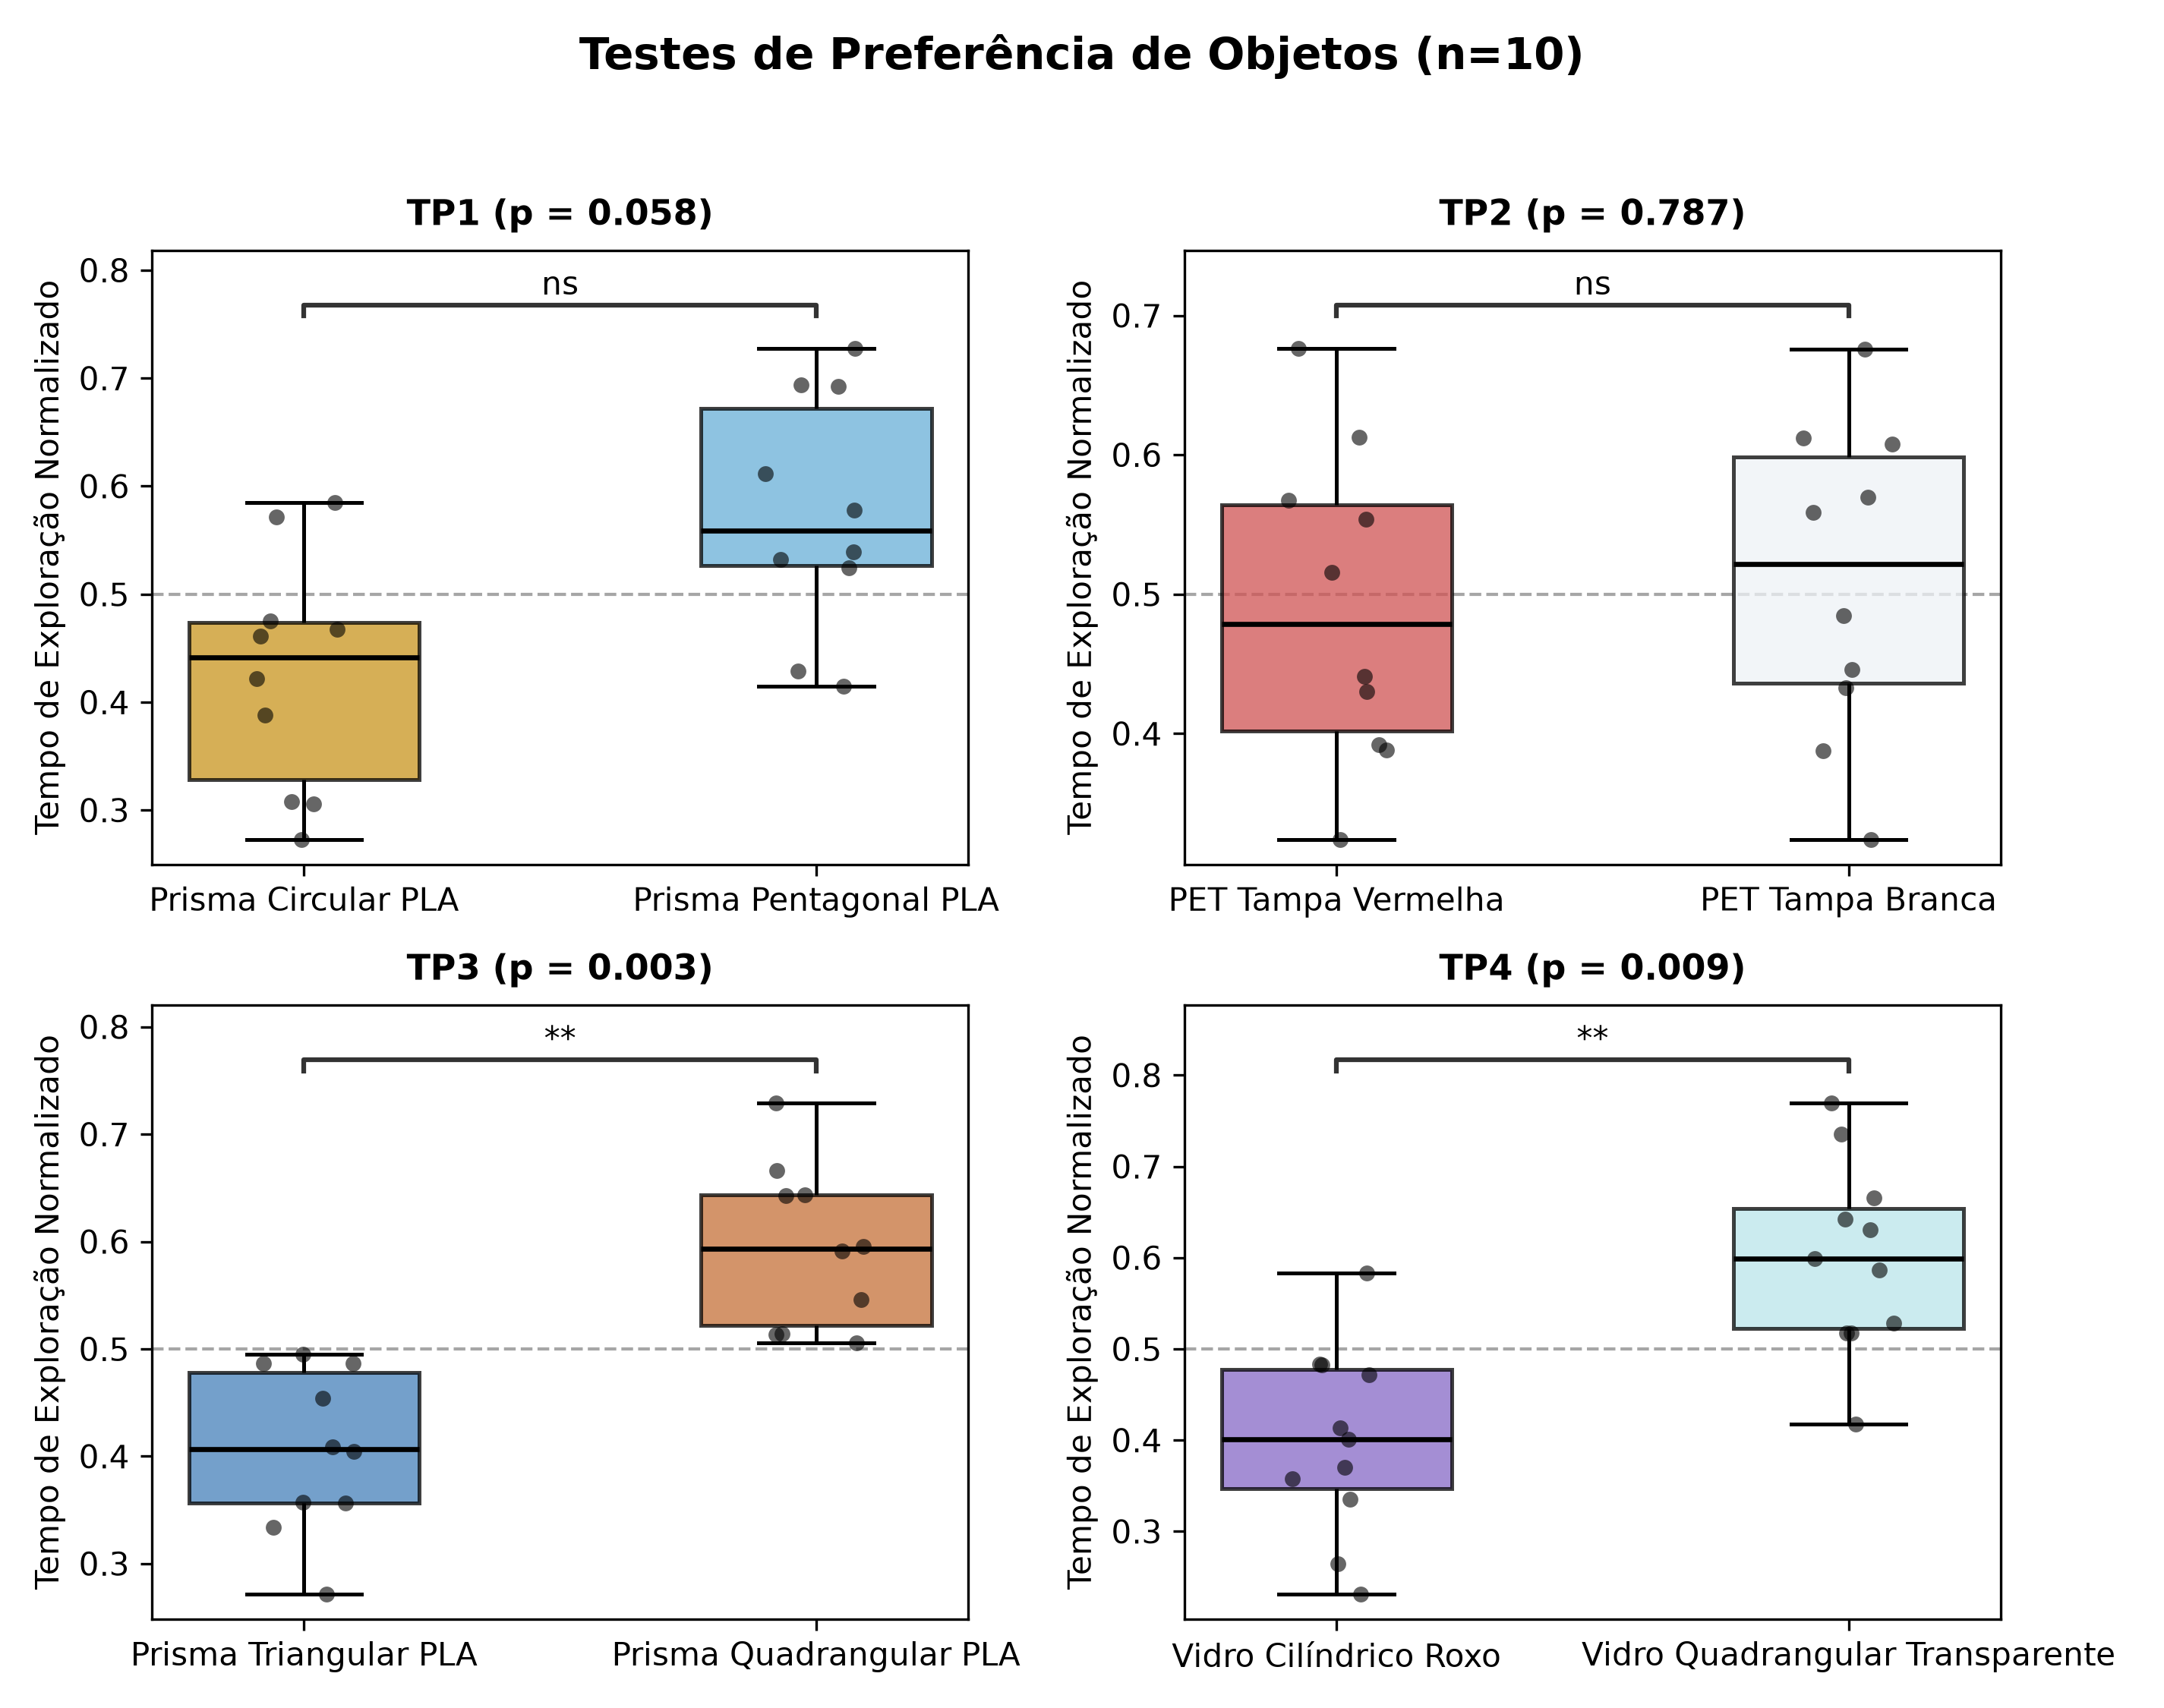
\includegraphics[width=0.9\textwidth]{grafico_preferencia_obj.png}
    \caption{Tempo relativo de exploração nos testes de preferência de objetos em animais \emph{naive}. A linha tracejada em $y = 0{,}50$ denota equivalência exploratória estrita (neutralidade). Notações nas chaves superiores referem-se a comparações pareadas intra-sujeito (ns = não significativo; * = $p < 0{,}05$; ** = $p < 0{,}01$).}
    \label{fig:teste_preferencia}
\end{figure}

Para assegurar que a neutralidade observada no Teste~2 não decorresse de apatia motora ou déficits de atenção, avaliou-se a proporção global de locomoção e repouso. Como demonstrado na \cref{fig:exploracao_repouso}, os índices de exploração e imobilidade foram homogêneos entre as quatro condições experimentais, confirmando que a simetria do par PET decorre de equivalência perceptual genuína.

\begin{figure}[!ht]
    \centering
    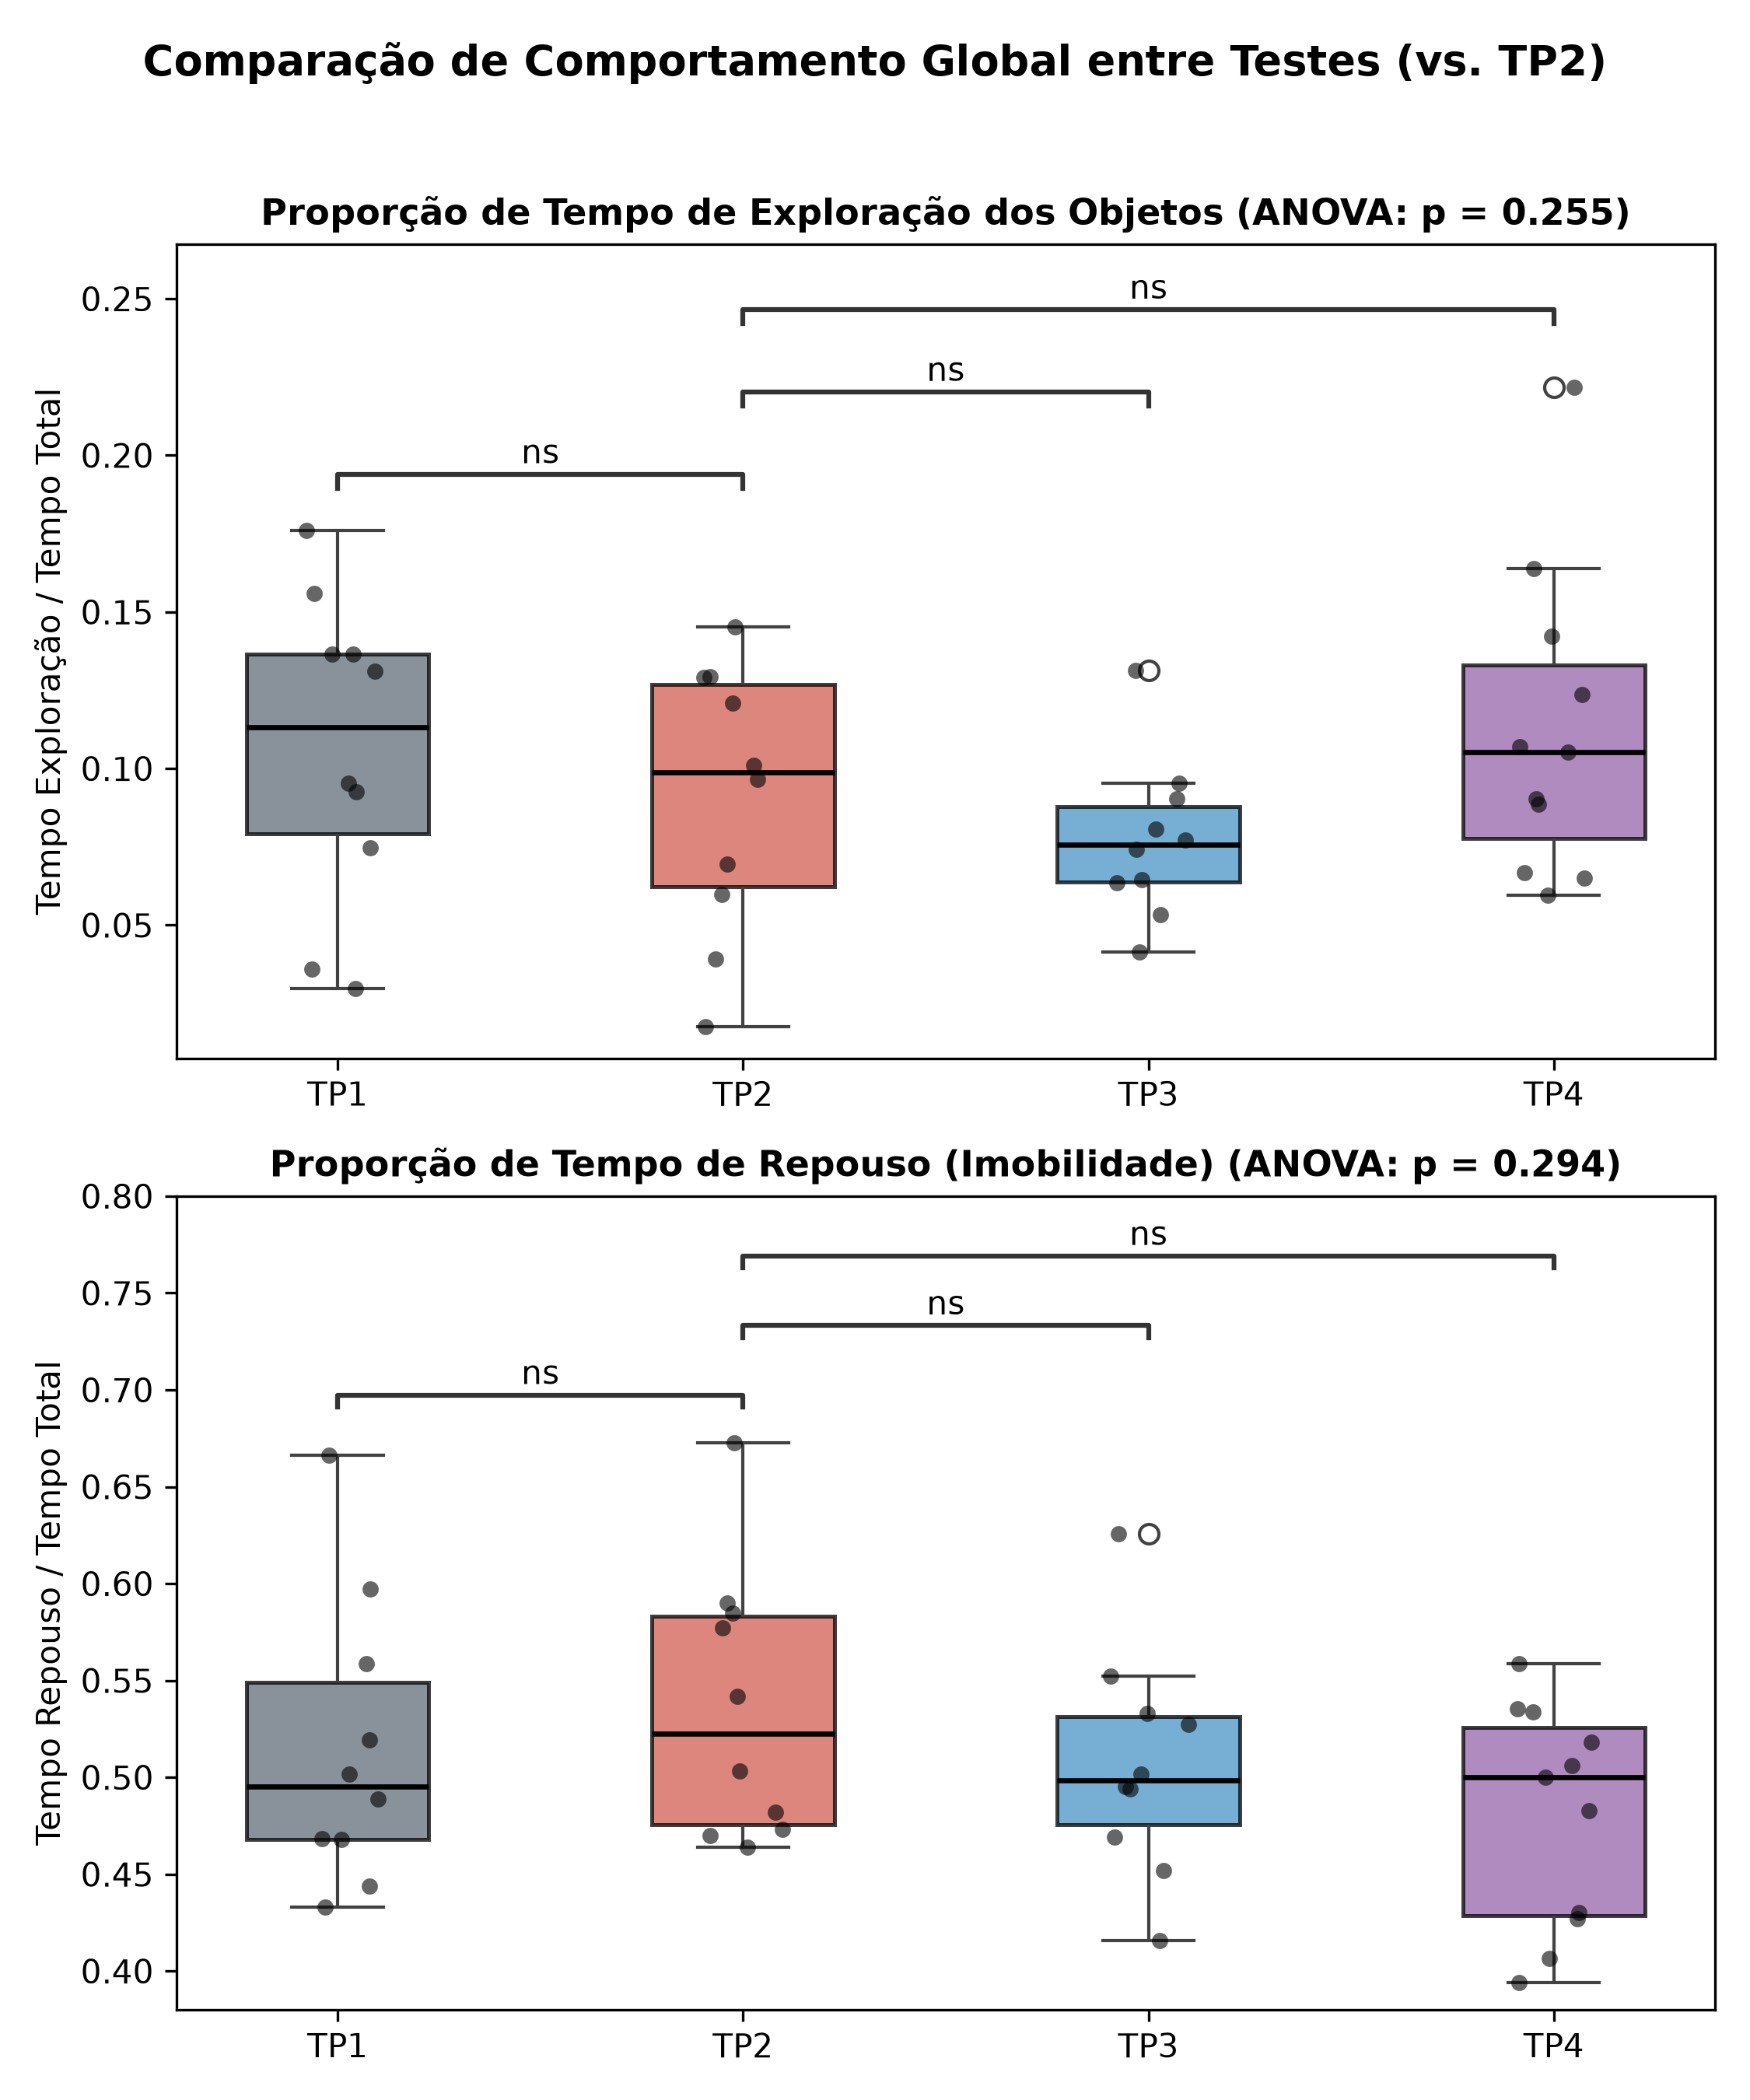
\includegraphics[width=0.78\textwidth]{grafico_exploracao_repouso_anova.png}
    \caption{Proporção do tempo de sessão devotada à exploração ativa e ao repouso motor nos quatro testes de preferência de objetos em animais \emph{naive}. As chaves indicam comparações pareadas frente ao Teste~2 (par selecionado).}
    \label{fig:exploracao_repouso}
\end{figure}

\chapter{Análise Comportamental Integrada dos Lotes Experimentais}

Os experimentos de condicionamento com microestimulação elétrica foram executados sequencialmente em coortes sucessivas de animais, consolidadas conforme a discriminação apresentada na \cref{tab:lotes_comportamento}.

\begin{table}[tbp]
    \centering
    \small
    \setlength{\tabcolsep}{3.5pt}
    \caption{Dados dos lotes de animais.}
    \label{tab:lotes_comportamento}
    \begin{adjustbox}{max width=0.95\textwidth}
        \begin{tabular}{cccc}
            \toprule
            \textbf{Lote de Animais}   & \textbf{$N$} & \textbf{Par de Objetos} & \textbf{Status dos Dados}   \\
            \midrule
            \#1                        & 3            & Vidro (TP4)             & Sem dados de video          \\
            \#2                        & 4            & Vidro (TP4)             & Com dados de video          \\
            \#3                        & 8            & Vidro (TP4)             & Com dados de video          \\
            \#4                        & 7            & PET (TP2)               & Com dados de video          \\
            \#5                        & 3            & PET (TP2)               & Dados de video não nomeados \\
            \#6                        & 16           & PET (TP2)               & Dados de video não nomeados \\
            \midrule
            \textbf{Total de Amostras} & \textbf{41}  &                         &                             \\
            \bottomrule
        \end{tabular}
    \end{adjustbox}
\end{table}

Em termos de integridade e transparência, cumpre salientar que dos 41 animais manipulados em bancada, apenas os lotes \#2, \#3 e \#4 dispõem de gravações de vídeo válidas e catalogadas que permitiram o rastreamento computacional por \textit{pose estimation} (Behavython/DeepLabCut). Os animais dos lotes \#1 (falha de aquisição de vídeo), \#5 e \#6 (incompatibilidade de rastreabilidade nos arquivos brutos) foram mantidos no registro histórico da bancada, mas excluídos das quantificações cinemáticas.

\section{Preferência Exploratória na Sessão Teste}

A investigação do efeito da microestimulação sobre a preferência na sessão de teste exige a consideração direta da ordem cronológica em que os ensaios foram realizados. Os lotes \#2 e \#3 foram conduzidos utilizando o par de estímulos de vidro (TP4). Como demonstrado na bateria de testes de preferência (\cref{tab:testes_preferencia}), os frascos de vidro induzem preferência inata pelo exemplar quadrangular transparente.

A distribuição de preferência dos lotes \#2 e \#3 é apresentada na \cref{fig:pref_lotes_vidro}, enquanto os dados do lote \#4 (frascos PET simétricos) são exibidos na \cref{fig:pref_lote_pet}. Os parâmetros descritivos e as estatísticas inferenciais de ambos os ensaios encontram-se sintetizados na \cref{tab:estatistica_preferencia_lotes}.

\begin{figure}[!ht]
    \centering
    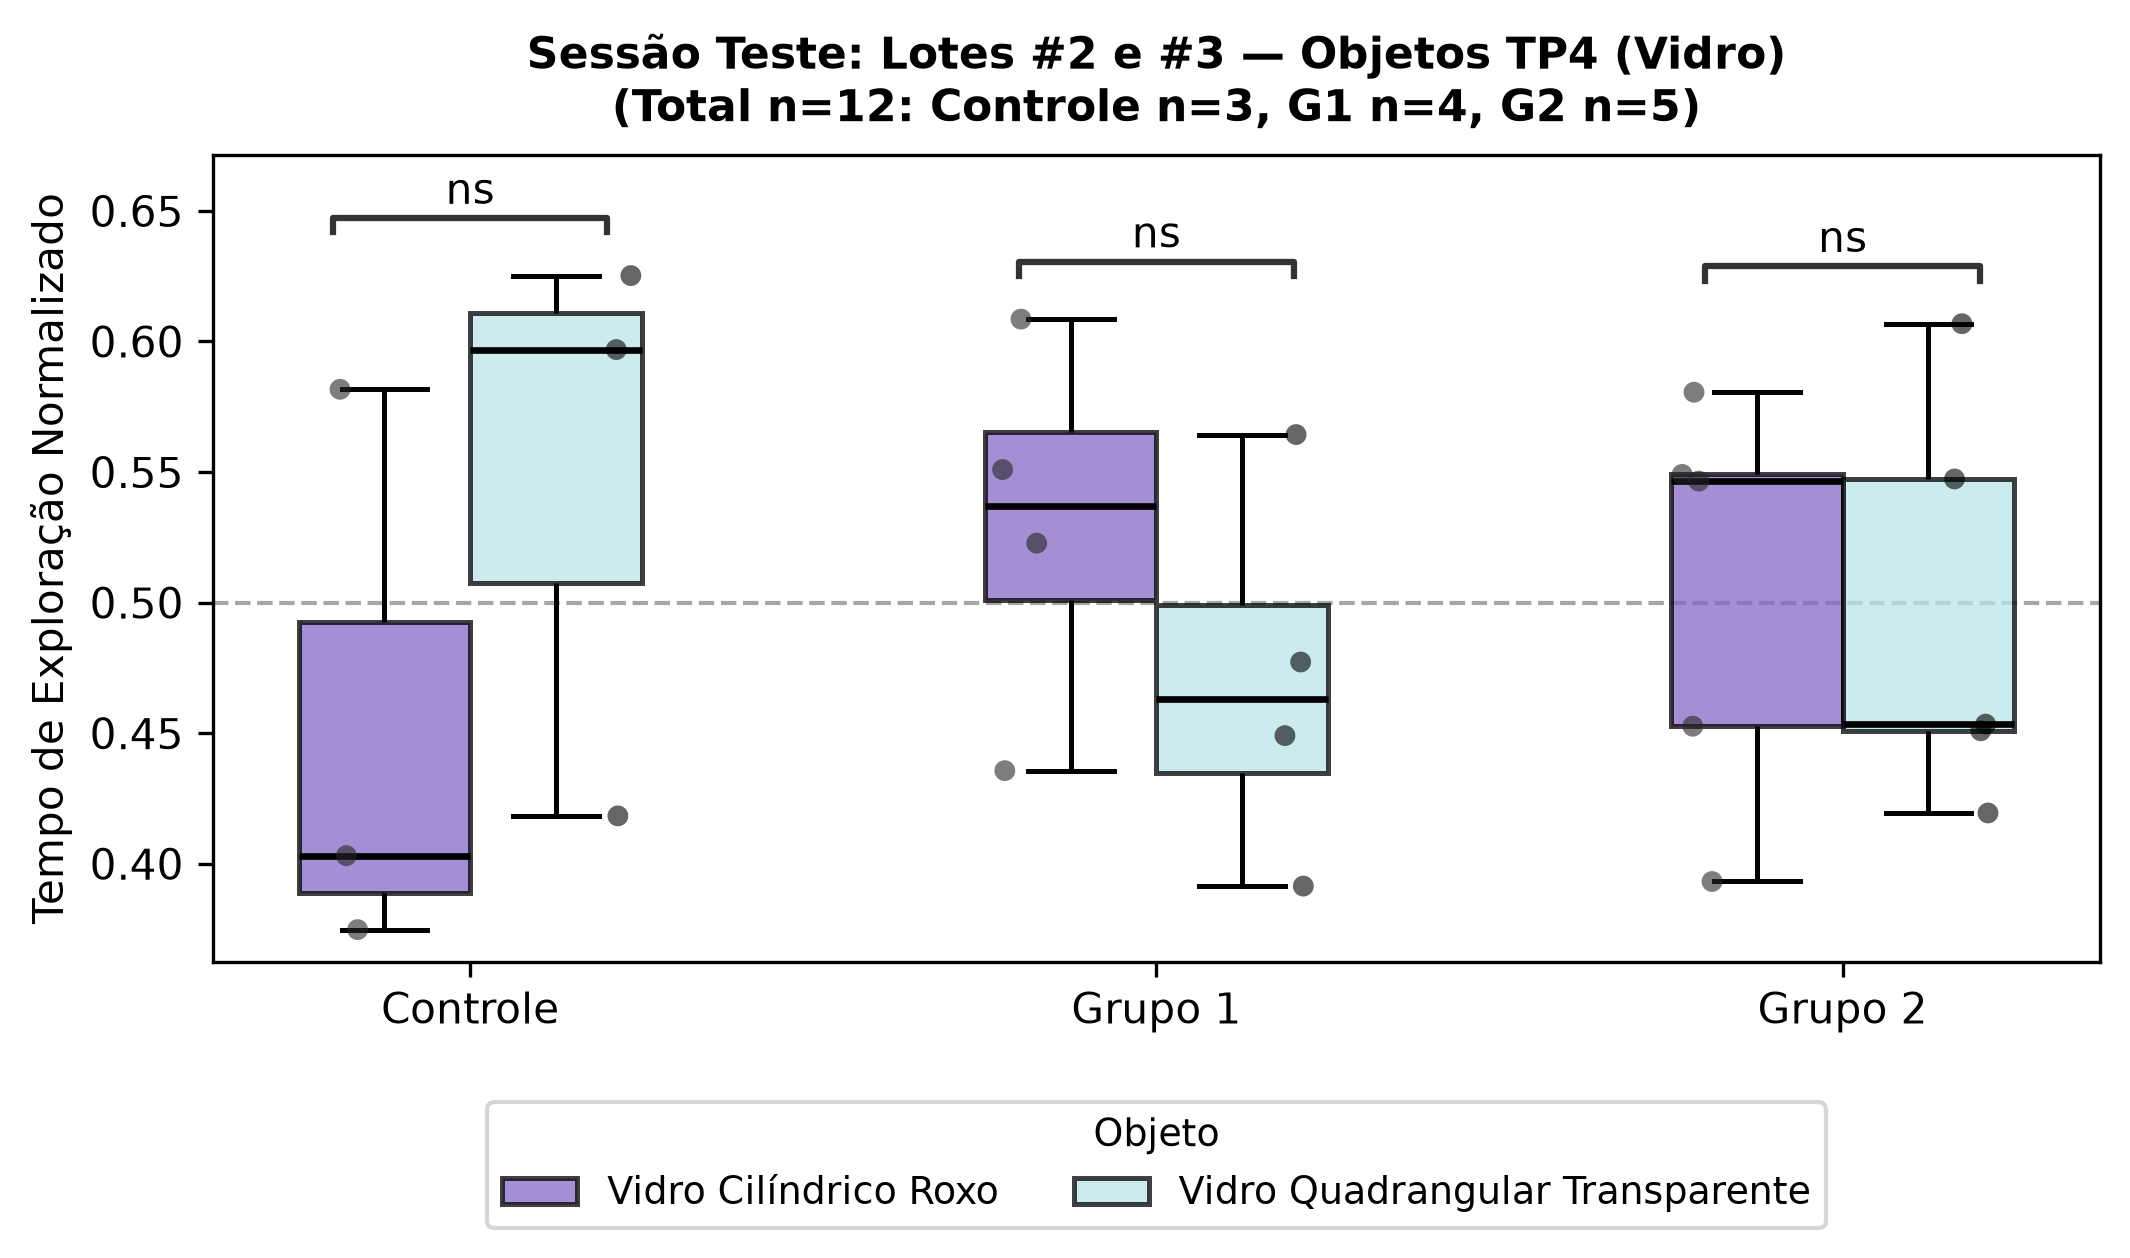
\includegraphics[width=0.75\textwidth]{grafico_comportamento_preferencia_lotes_vidro.png}
    \caption{Distribuição da proporção do tempo de exploração entre o vidro cilíndrico roxo e o vidro quadrangular transparente durante a sessão de teste nos lotes \#2 e \#3, estratificada por grupo experimental (Controle, Grupo~1 e Grupo~2). Boxplots acompanhados de dispersão individual de dados (stripplot). A linha tracejada em $0{,}50$ indica neutralidade de exploração.}
    \label{fig:pref_lotes_vidro}
\end{figure}

\begin{figure}[!ht]
    \centering
    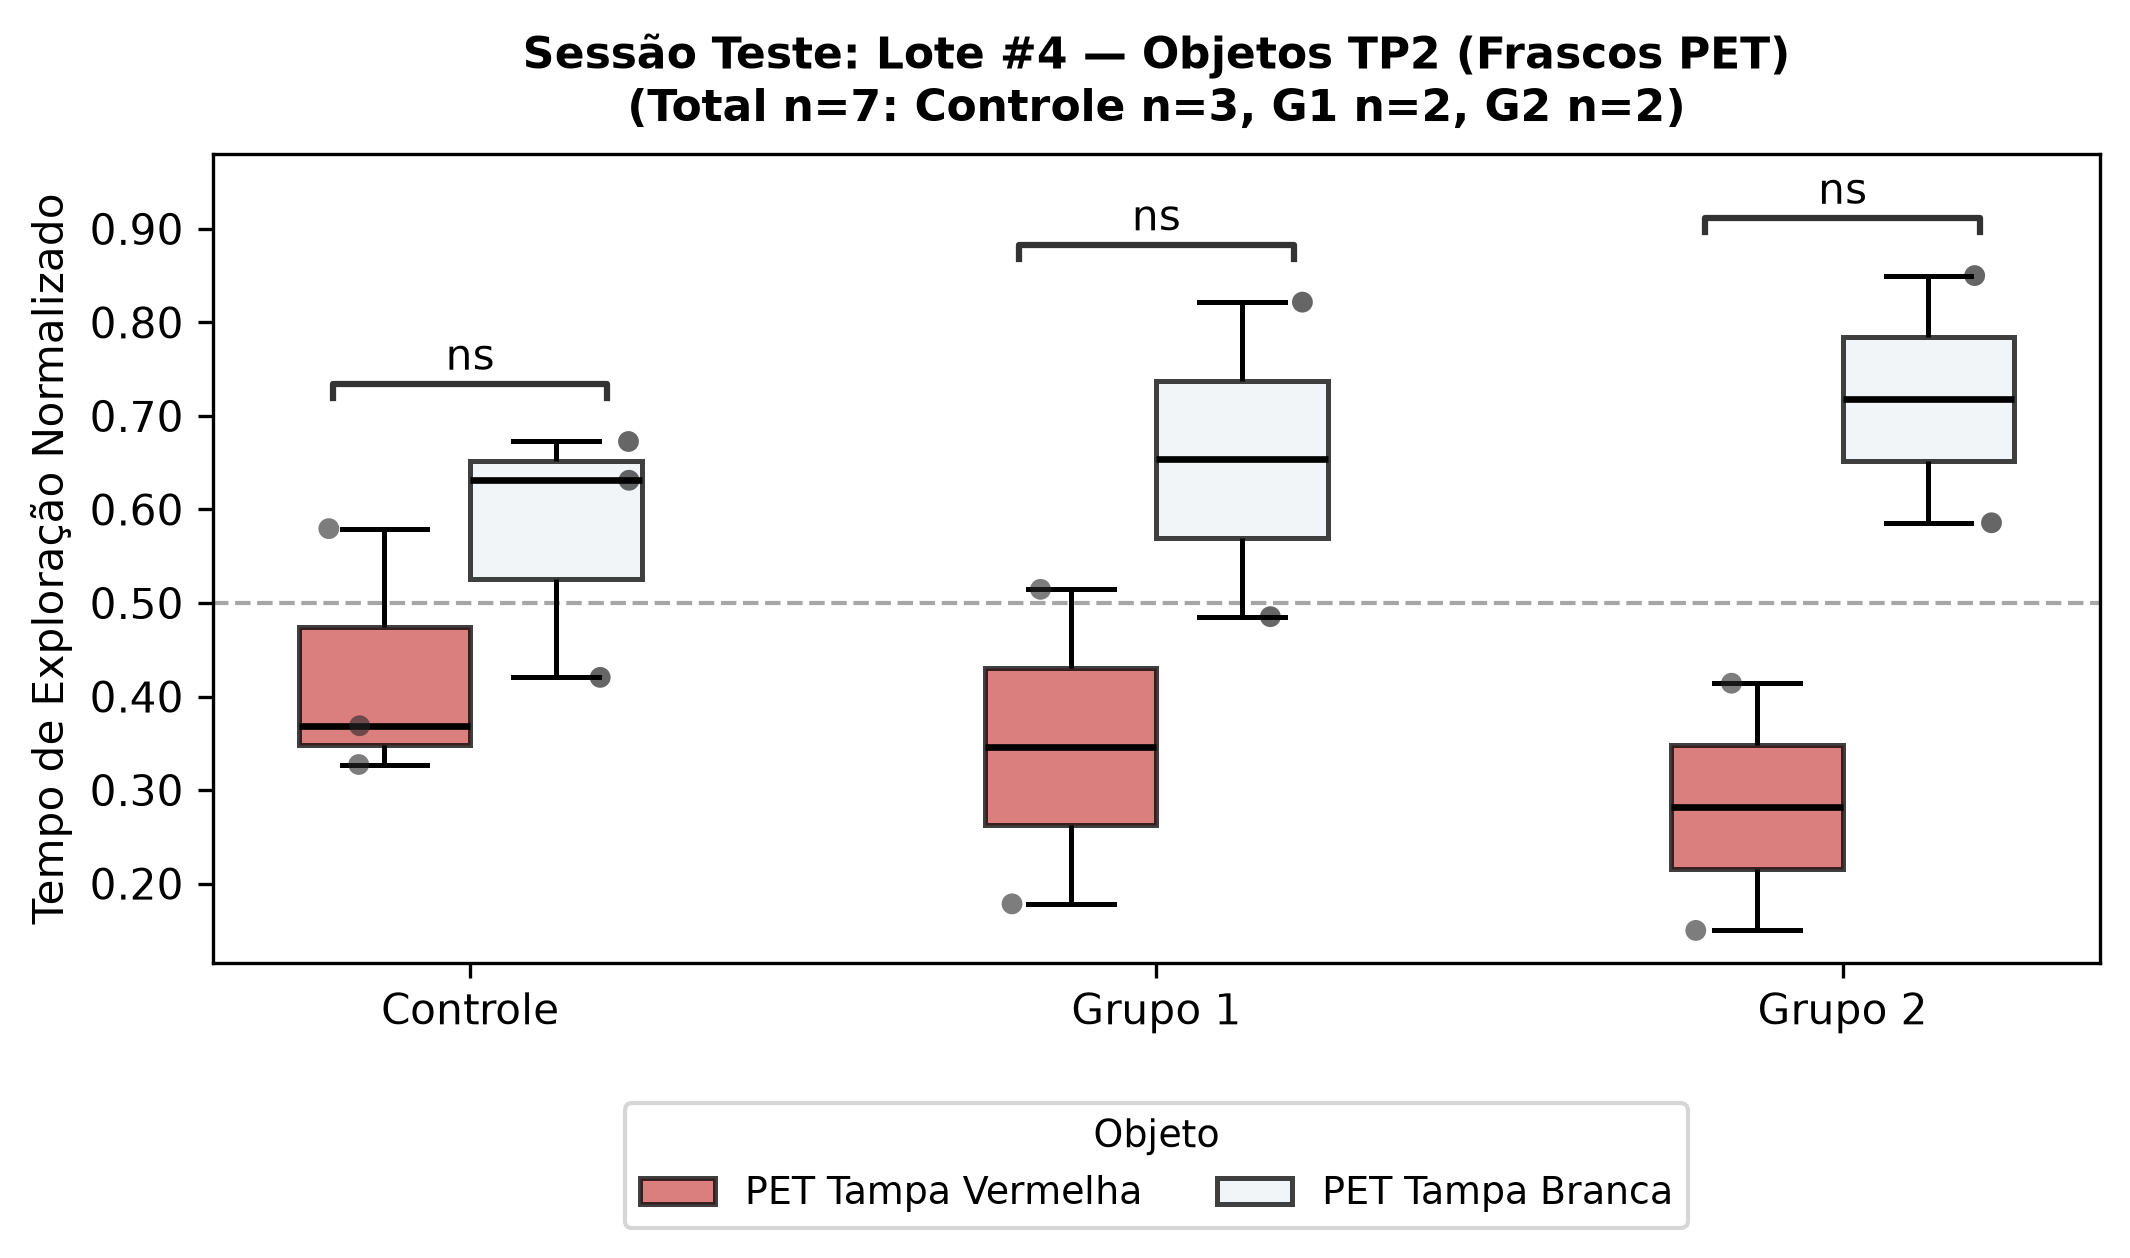
\includegraphics[width=0.75\textwidth]{grafico_comportamento_preferencia_lote_pet.png}
    \caption{Distribuição da proporção de exploração entre o frasco PET com tampa vermelha e com tampa branca durante a sessão de teste no lote \#4, estratificada por grupo experimental (Controle, Grupo~1 e Grupo~2). A linha tracejada em $0{,}50$ representa a linha de neutralidade.}
    \label{fig:pref_lote_pet}
\end{figure}

\begin{table}[tbp]
    \centering
    \small
    \setlength{\tabcolsep}{3.5pt}
    \caption{Parâmetros estatísticos descritivos e inferenciais da exploração pareada de objetos na sessão teste.}
    \label{tab:estatistica_preferencia_lotes}
    \begin{adjustbox}{max width=0.95\textwidth}
        \begin{tabular}{llcccc}
            \toprule
            \textbf{Lotes} & \textbf{Grupo} & \textbf{$n$} & \textbf{Objeto Esquerdo} & \textbf{Objeto Direito} & \textbf{Teste $t$ ($p$-valor)}    \\
            \midrule
            \multirow{3}{*}{\shortstack[l]{\textbf{Lotes \#2 e \#3}\\(Vidro: TP4)}}
                           & Controle       & 3            & $0{,}453 \pm 0{,}112$    & $0{,}547 \pm 0{,}112$   & $t(2) = -0{,}723$ ($p = 0{,}545$) \\
                           & Grupo 1        & 4            & $0{,}529 \pm 0{,}072$    & $0{,}471 \pm 0{,}072$   & $t(3) = 0{,}819$ ($p = 0{,}473$)  \\
                           & Grupo 2        & 5            & $0{,}504 \pm 0{,}078$    & $0{,}496 \pm 0{,}078$   & $t(4) = 0{,}126$ ($p = 0{,}906$)  \\
            \midrule
            \multirow{3}{*}{\shortstack[l]{\textbf{Lote \#4}\\(PET: TP2)}}
                           & Controle       & 3            & $0{,}425 \pm 0{,}135$    & $0{,}575 \pm 0{,}135$   & $t(2) = -0{,}958$ ($p = 0{,}439$) \\
                           & Grupo 1        & 2            & $0{,}347 \pm 0{,}238$    & $0{,}653 \pm 0{,}238$   & $t(1) = -0{,}913$ ($p = 0{,}529$) \\
                           & Grupo 2        & 2            & $0{,}282 \pm 0{,}187$    & $0{,}718 \pm 0{,}187$   & $t(1) = -1{,}649$ ($p = 0{,}347$) \\
            \bottomrule
        \end{tabular}
    \end{adjustbox}
    \vspace{0.2em}
    \begin{minipage}{0.95\textwidth}
        \footnotesize \textbf{Nota:} Valores reportados como média $\pm$ desvio padrão da proporção de tempo exploratório ($t_{\text{objeto}} / t_{\text{exploração total}}$). Nos lotes \#2 e \#3 os objetos correspondem a Vidro Cilíndrico Roxo (esq.) e Vidro Quadrangular Transparente (dir.); no lote \#4 correspondem a Frasco PET com tampa vermelha (esq.) e tampa branca (dir.). As comparações inferenciais referem-se ao teste $t$ de Student pareado bicaudal intra-sujeito.
    \end{minipage}
\end{table}


Conforme evidenciado visualmente pelas barras de significância e confirmado na \cref{tab:estatistica_preferencia_lotes}, nenhum dos grupos experimentais manifestou divergência estatisticamente significante entre os dois objetos na sessão teste. Contudo, as razões epistemológicas dessa ausência de significância diferem fundamentalmente entre as duas coortes:

\subsection{Problema Metodológico e Inviabilidade de Normalização dos Lotes \#2 e \#3}
Nos lotes \#2 e \#3 (\cref{fig:pref_lotes_vidro}), a igualdade aparente de exploração média entre os estímulos reflete a sobreposição de um viés sensorial preexistente da garrafa de vidro sobre a modulação mnemônica tênue gerada pela estimulação em malha aberta. Na literatura de neurobiologia do comportamento \cite{dix1999, leger2013}, questiona-se frequentemente se esses dados poderiam ser aproveitados mediante normalizações algébricas \emph{post-hoc} — por exemplo, subtraindo o Índice de Discriminação basal obtido com animais \emph{naive}.

Fundamentos científicos clássicos refutam essa correção: (i) a preferência inata por saliência visual ou tátil não é um escalar constante, variando dinamicamente com a habituação intensesão e com a microestrutura dos episódios de contato \cite{ennaceur1988}; (ii) a interação entre traço mnemônico hipocampal e atratividade sensorial viola os pressupostos de aditividade linear de modelos corretivos; e (iii) a propagação de incertezas da linha de base expande o erro padrão da média, destruindo o poder estatístico residual do ensaio. Assim, em conformidade com o rigor de boas práticas laboratoriais, os lotes \#2 e \#3 devem ser classificados como etapa de desenvolvimento experimental e prova de estabilidade motora, não devendo compor a análise inferencial confirmatória de discriminação associativa.


\subsection{Subdimensionamento Amostral no Lote \#4}
No lote \#4 (\cref{fig:pref_lote_pet}), a utilização de frascos PET eliminou os vieses intrínsecos de material. Os dados descritivos apontam que os animais estimulados direcionaram frações superiores de exploração ao frasco de tampa branca, em contraste com a distribuição do grupo controle (\cref{tab:estatistica_preferencia_lotes}). Todavia, as comparações pareadas intra-sujeito não alcançaram significância estatística.

Esse resultado decorre fundamentalmente do tamanho amostral diminuto ($n = 2$ a $3$ sujeitos por célula experimental). Com essa densidade amostral, o poder estatístico (\emph{power}) a priori para identificar tamanhos de efeito intermediários é inferior a $20\%$, elevando drasticamente o risco de erro tipo II (falso negativo). Logo, embora o lote \#4 forneça a base metodológica correta, os achados devem ser interpretados estritamente como indicativos preliminares de viabilidade instrumental, sendo cientificamente infundado extrapolar essas estimativas pontuais como representativas de toda a população de camundongos C57BL/6.

\section{Dinâmica de Movimento entre Grupos Experimentais}

Para determinar se a microestimulação de CA3 em malha aberta afeta a capacidade locomotora basal, induz quadros de sedação ou produz imobilidade comportamental (\emph{freezing}), analisou-se a partição temporal da atividade dos animais ao longo de todas as sessões monitoradas. A proporção de exploração ativa dos objetos está representada na \cref{fig:grupos_exploracao}, enquanto o tempo em repouso é ilustrado na \cref{fig:grupos_repouso}. Os parâmetros descritivos agregados e as estatísticas dos modelos de análise de variância constam na \cref{tab:estatistica_grupos_movimento}.

\begin{figure}[!ht]
    \centering
    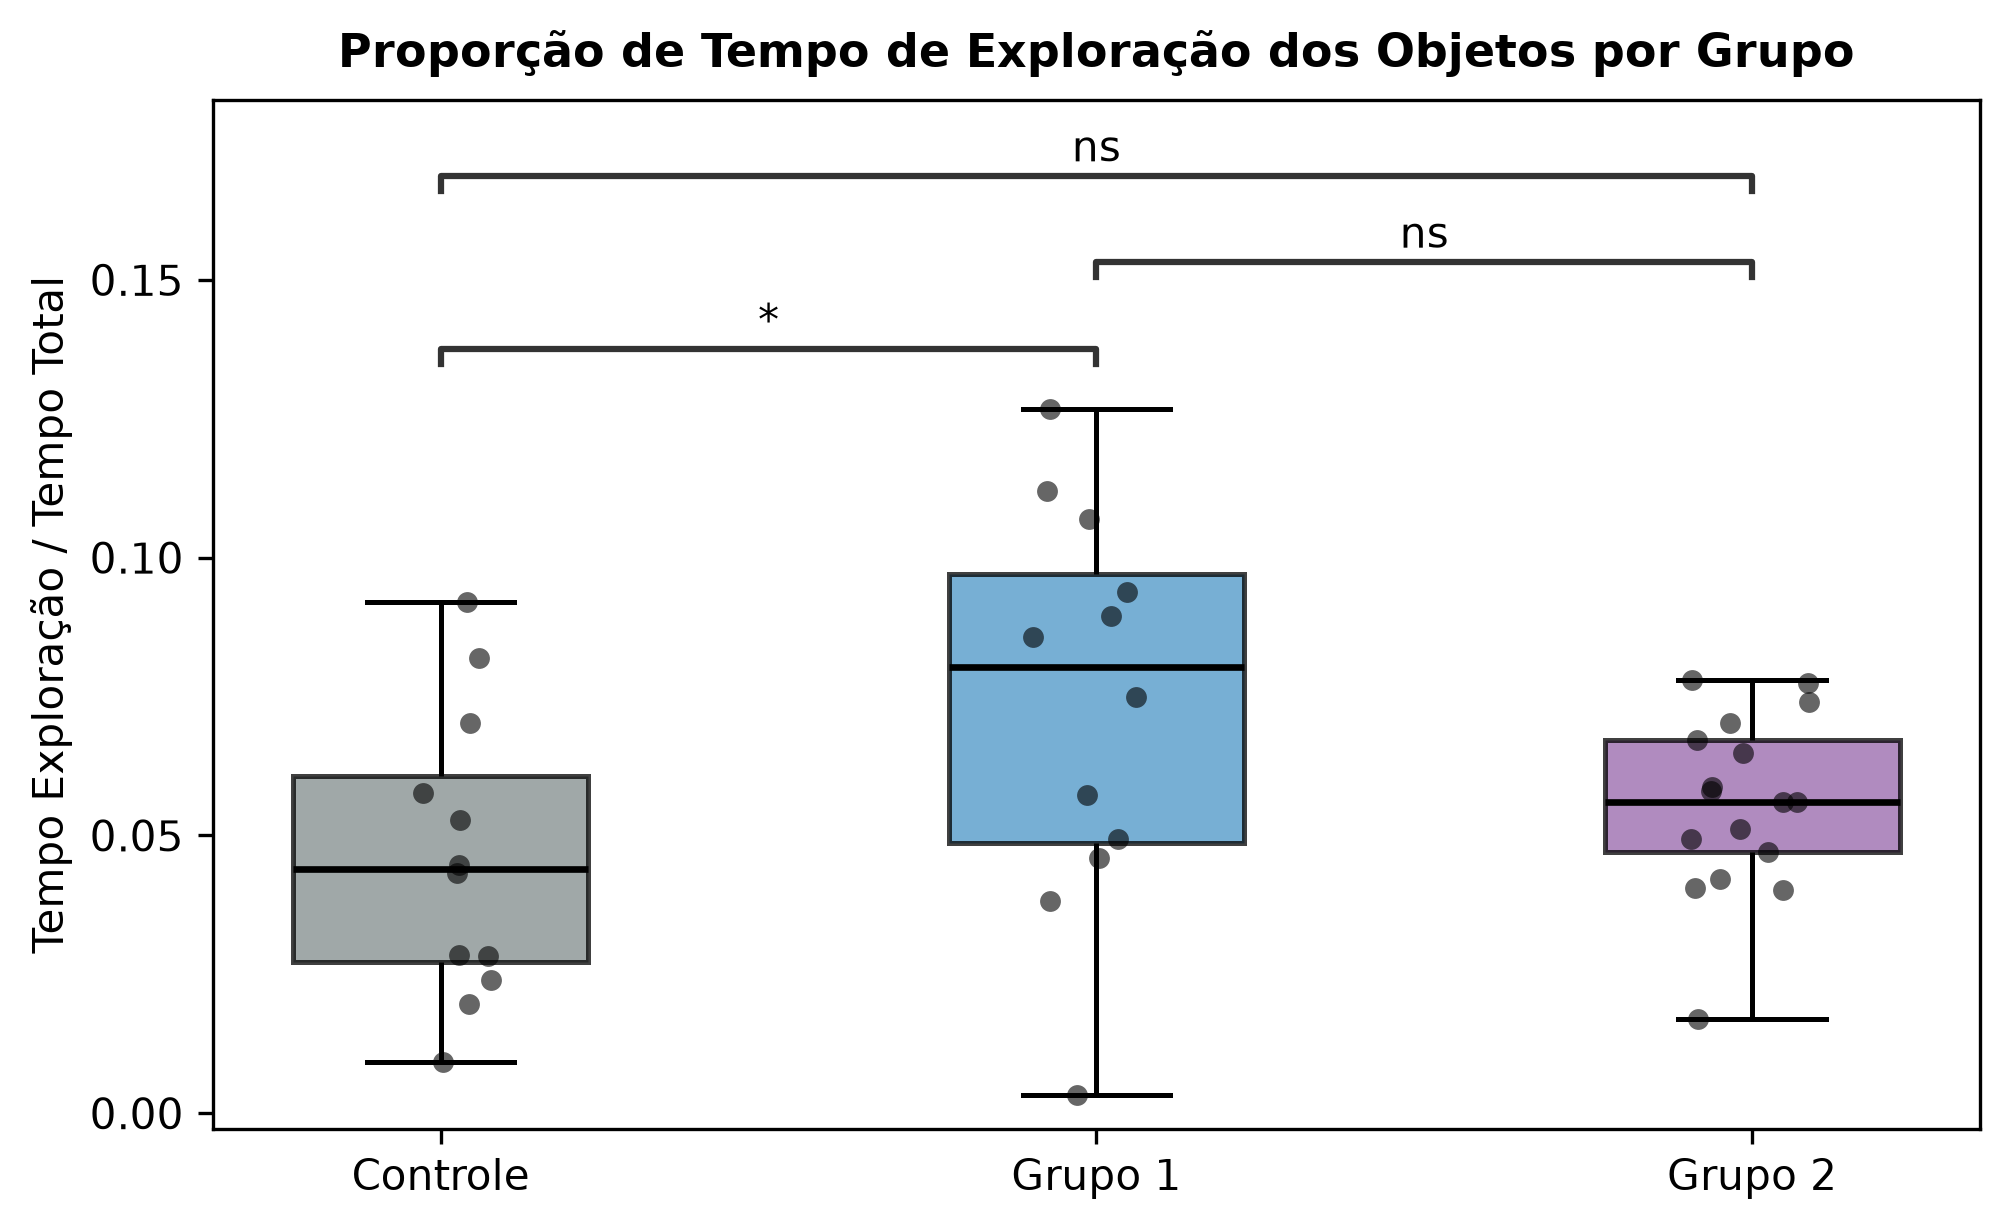
\includegraphics[width=0.68\textwidth]{grafico_comportamento_grupos_exploracao.png}
    \caption{Proporção do tempo total de sessão dedicada à exploração ativa dos objetos por grupo experimental (Controle, Grupo~1 e Grupo~2), agregando todos os lotes com registro de vídeo. A barra superior denota diferença estatisticamente significante (* = $p < 0{,}05$) entre o grupo Controle e o Grupo~1.}
    \label{fig:grupos_exploracao}
\end{figure}

\begin{figure}[!ht]
    \centering
    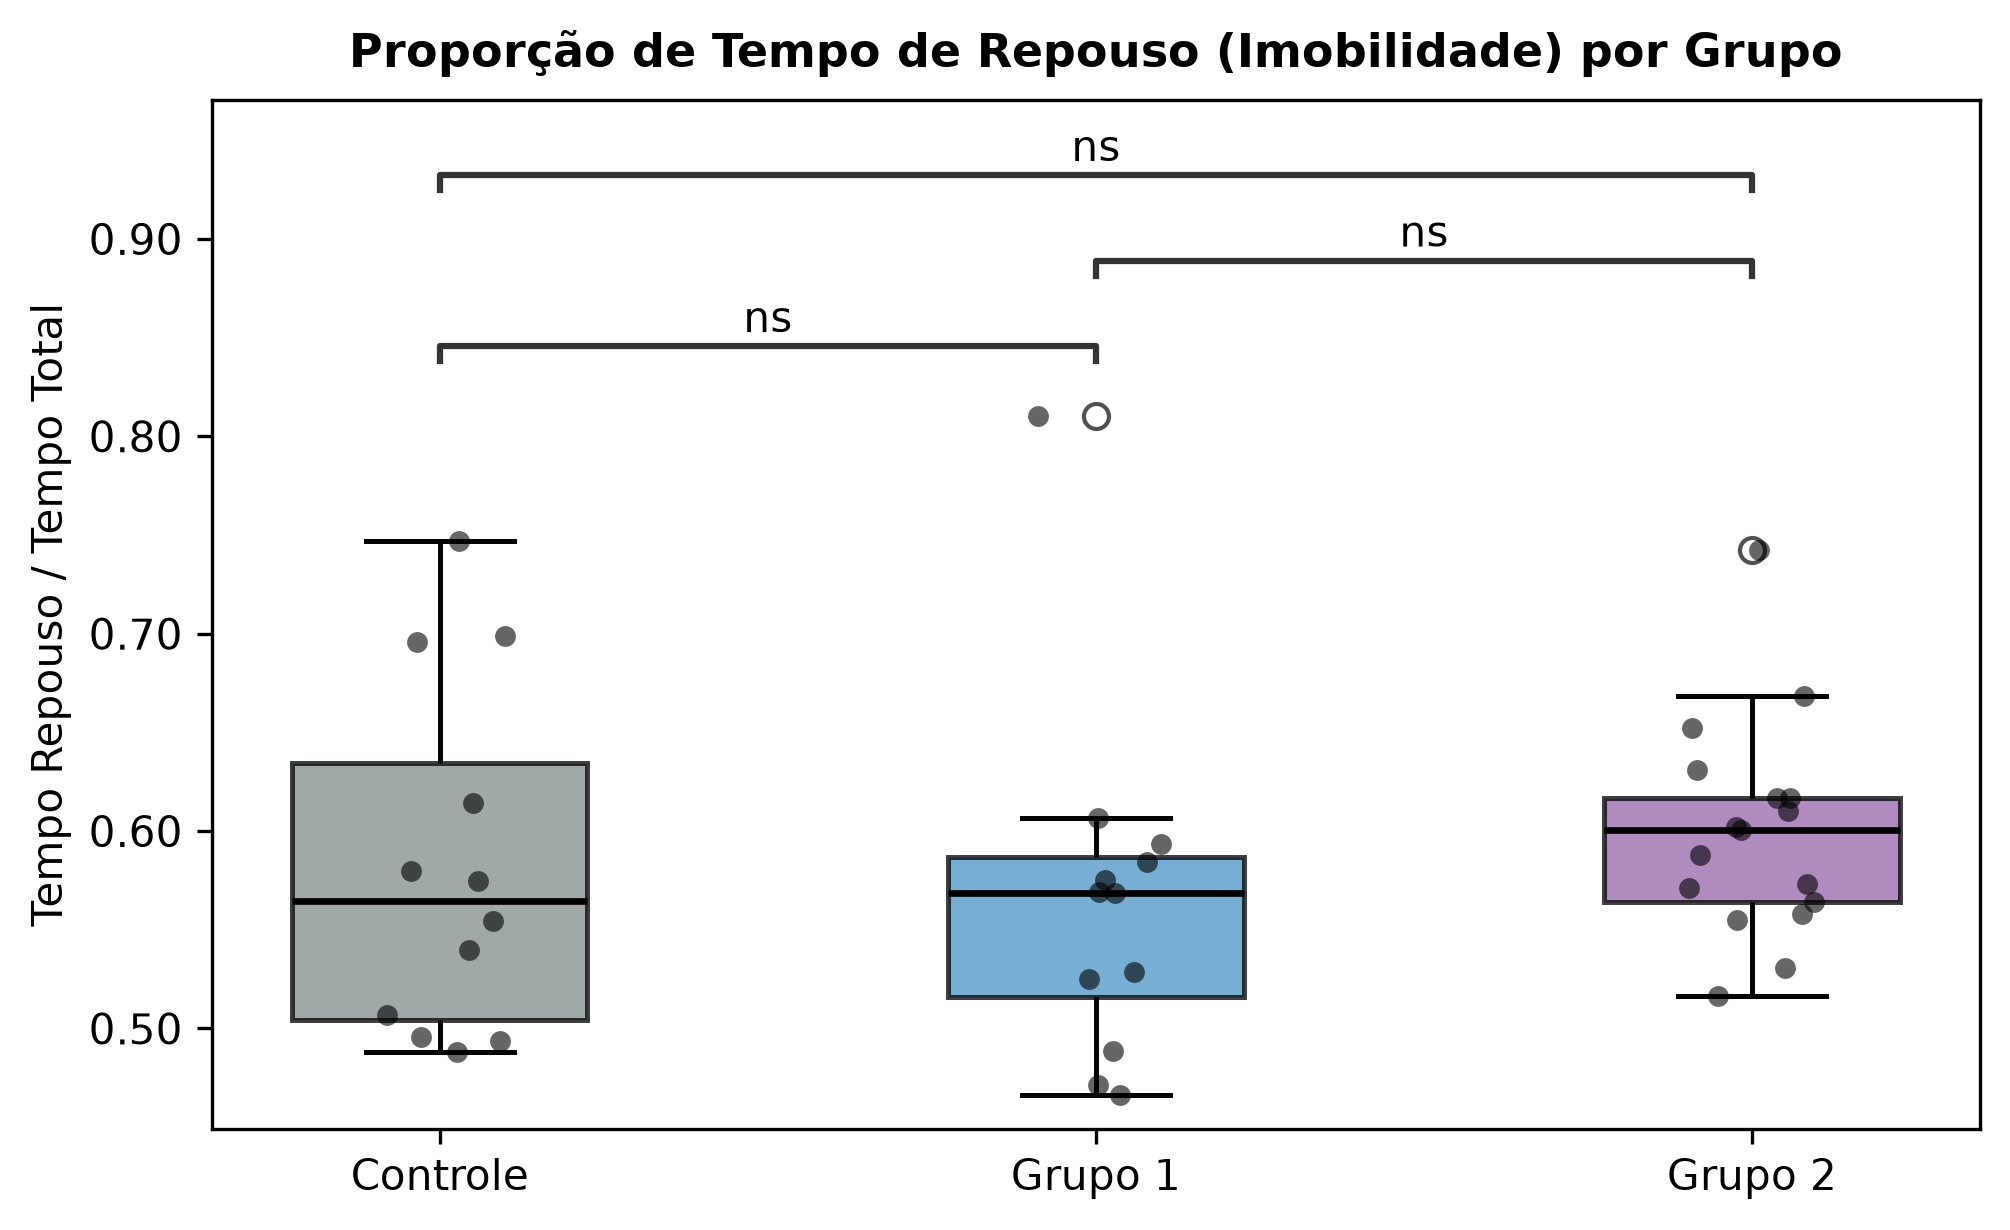
\includegraphics[width=0.68\textwidth]{grafico_comportamento_grupos_repouso.png}
    \caption{Proporção do tempo de sessão devotada ao repouso motor (imobilidade) por grupo experimental (Controle, Grupo~1 e Grupo~2). As notações indicam ausência de diferenças significantes (ns = $p \ge 0{,}05$).}
    \label{fig:grupos_repouso}
\end{figure}

\begin{table}[tbp]
    \centering
    \small
    \setlength{\tabcolsep}{4.5pt}
    \caption{Parâmetros de mobilidade motora e atividade geral discriminados por grupo experimental (todos os lotes agregados).}
    \label{tab:estatistica_grupos_movimento}
    \begin{adjustbox}{max width=0.95\textwidth}
        \begin{tabular}{lcccc}
            \toprule
            \textbf{Grupo} & \textbf{Sessões ($N$)} & \textbf{Exploração ($t_{\text{exp}}/t_{\text{tot}}$)} & \textbf{Repouso ($t_{\text{rep}}/t_{\text{tot}}$)} & \textbf{Movimento ($t_{\text{mov}}/t_{\text{tot}}$)} \\
            \midrule
            Controle       & 12                     & $0{,}046 \pm 0{,}026$                                 & $0{,}582 \pm 0{,}089$                              & $0{,}372 \pm 0{,}083$                                \\
            Grupo 1        & 12                     & $0{,}074 \pm 0{,}036$                                 & $0{,}566 \pm 0{,}091$                              & $0{,}361 \pm 0{,}082$                                \\
            Grupo 2        & 17                     & $0{,}056 \pm 0{,}016$                                 & $0{,}600 \pm 0{,}055$                              & $0{,}344 \pm 0{,}052$                                \\
            \midrule
            \textbf{ANOVA} & 41                     & $F = 3{,}56$ ($p = 0{,}038$)                          & $F = 0{,}70$ ($p = 0{,}502$)                       & $F = 0{,}55$ ($p = 0{,}582$)                         \\
            \bottomrule
        \end{tabular}
    \end{adjustbox}
    \vspace{0.2em}
    \begin{minipage}{0.95\textwidth}
        \footnotesize \textbf{Nota:} Média $\pm$ desvio padrão. Graus de liberdade: $F(2, 38)$. Comparações \emph{post-hoc} para exploração: Controle vs. Grupo~1 ($t = -2{,}18$, $p = 0{,}041$); Controle vs. Grupo~2 ($t = -1{,}26$, $p = 0{,}217$); Grupo~1 vs. Grupo~2 ($t = 1{,}84$, $p = 0{,}078$).
    \end{minipage}
\end{table}


Os resultados evidenciam que o Grupo~1 apresentou engajamento exploratório significativamente superior ao do grupo Controle (\cref{fig:grupos_exploracao}), sugerindo que o padrão temporal específico administrado a essa coorte atuou facilitando a prontidão investigativa direcionada aos alvos físicos. O Grupo~2 situou-se em nível intermediário, sem separação formal em relação ao controle.

Em contrapartida, a fração de repouso comportamental manteve-se inalterada entre as três condições (\cref{fig:grupos_repouso,tab:estatistica_grupos_movimento}). A preservação estrita dos níveis de imobilidade descarta a hipótese de que a estimulação tenha desencadeado episódios epilépticos subclínicos, sedação inespecífica ou reações paralisantes de medo. O aumento na exploração no Grupo~1 reflete, portanto, uma redistribuição seletiva da atenção ativa dentro da arena, e não uma alteração na motilidade espontânea global.

\section{Evolução Longitudinal do Movimento ao Longo das Etapas}

A estabilidade longitudinal da locomoção e do impulso exploratório foi avaliada ao longo das fases sequenciais de Treino~1, Treino~2 e Teste, com vistas a descartar habituação excessiva ou fadiga acumulada decorrente das conexões mecânicas do cabo de estimulação. As trajetórias temporais de exploração e repouso são exibidas nas \cref{fig:etapas_exploracao,fig:etapas_repouso}, respectivamente, com quantificação paramétrica tabulada na \cref{tab:estatistica_etapas_movimento}.

\begin{figure}[!ht]
    \centering
    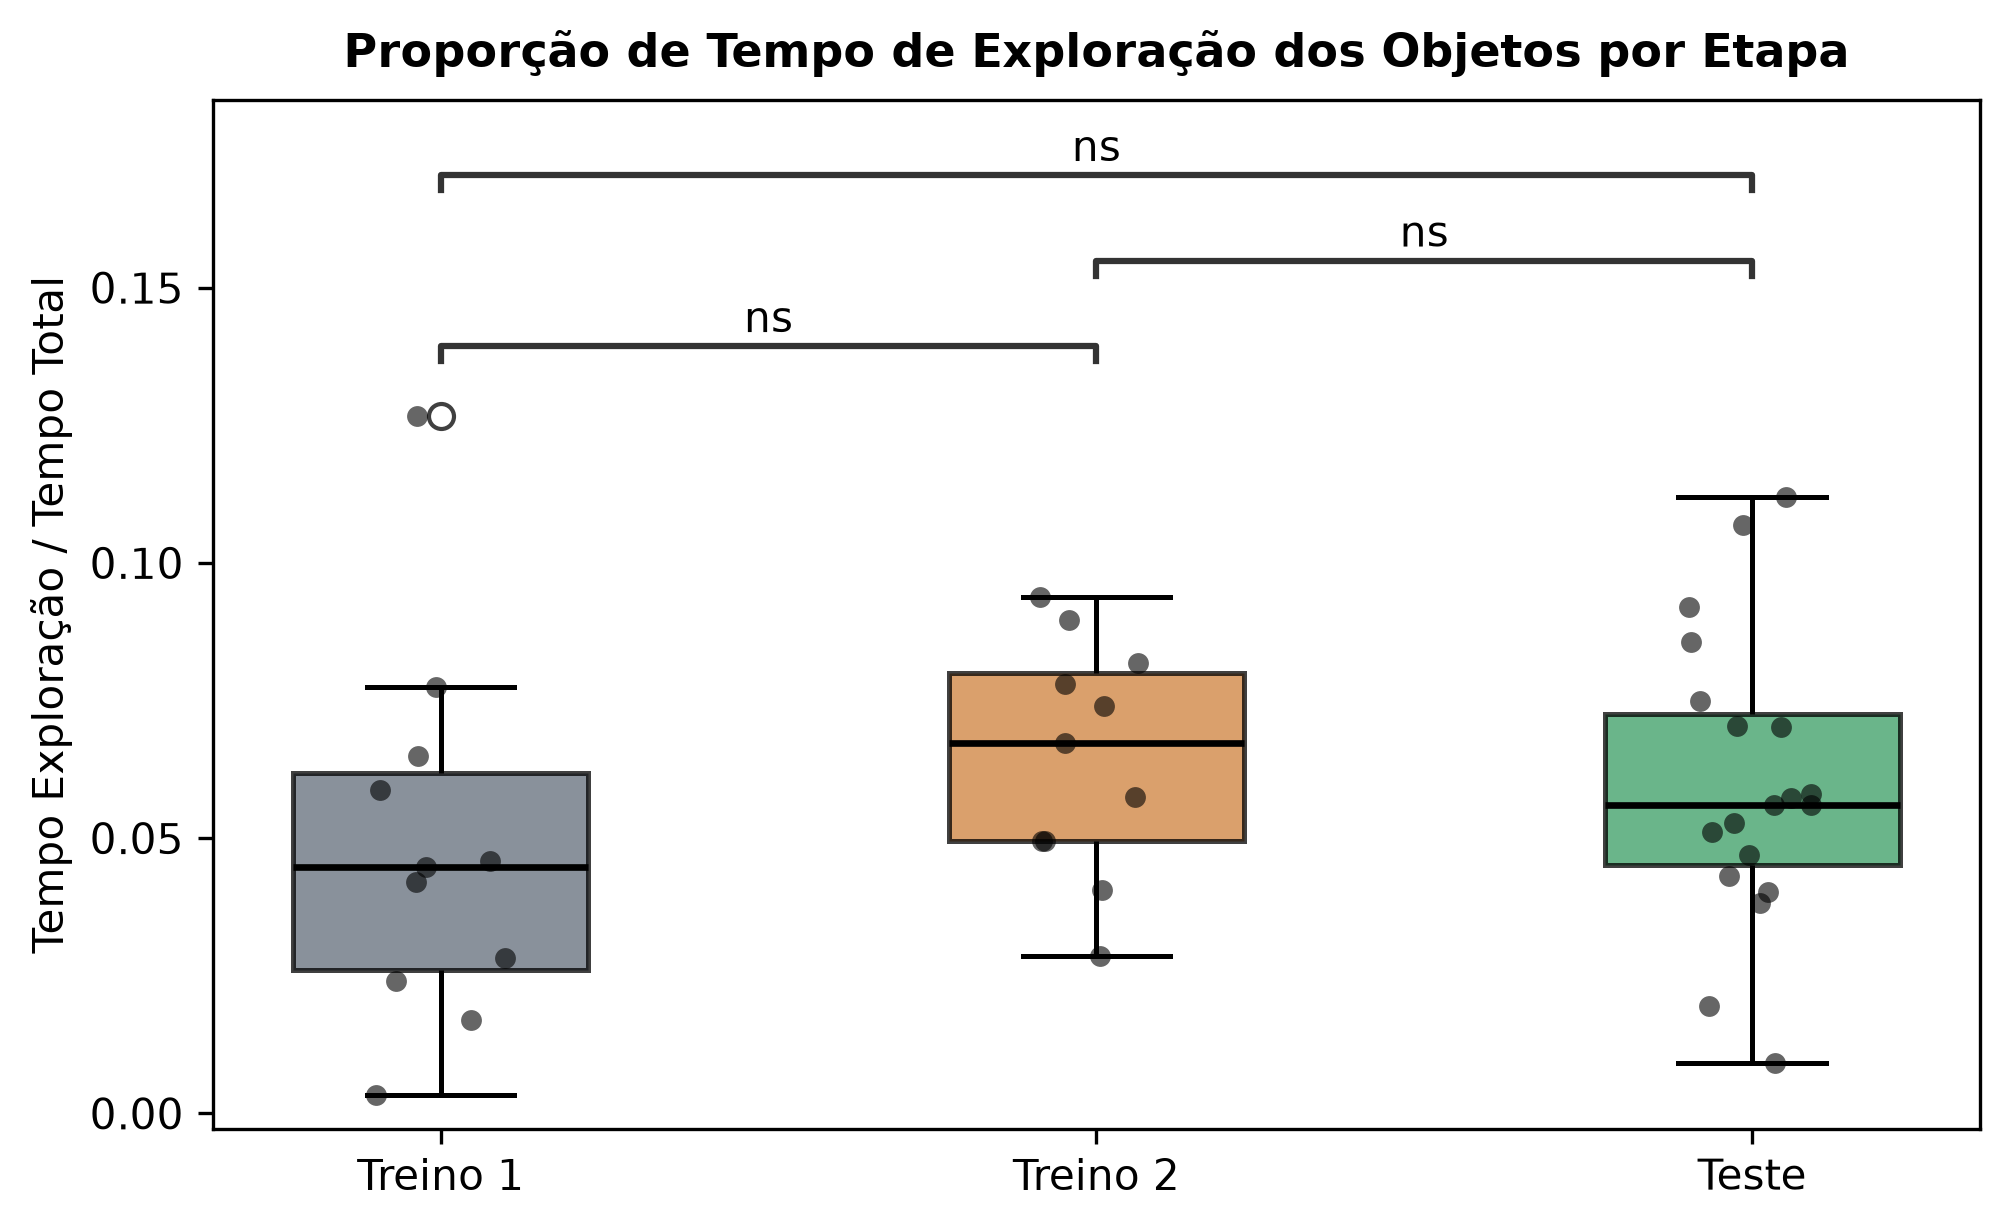
\includegraphics[width=0.68\textwidth]{grafico_comportamento_etapas_exploracao.png}
    \caption{Proporção de tempo dedicada à exploração ativa dos estímulos ao longo das etapas consecutivas de Treino~1, Treino~2 e Teste. As barras superiores indicam comparações bivariadas não significantes (ns).}
    \label{fig:etapas_exploracao}
\end{figure}

\begin{figure}[!ht]
    \centering
    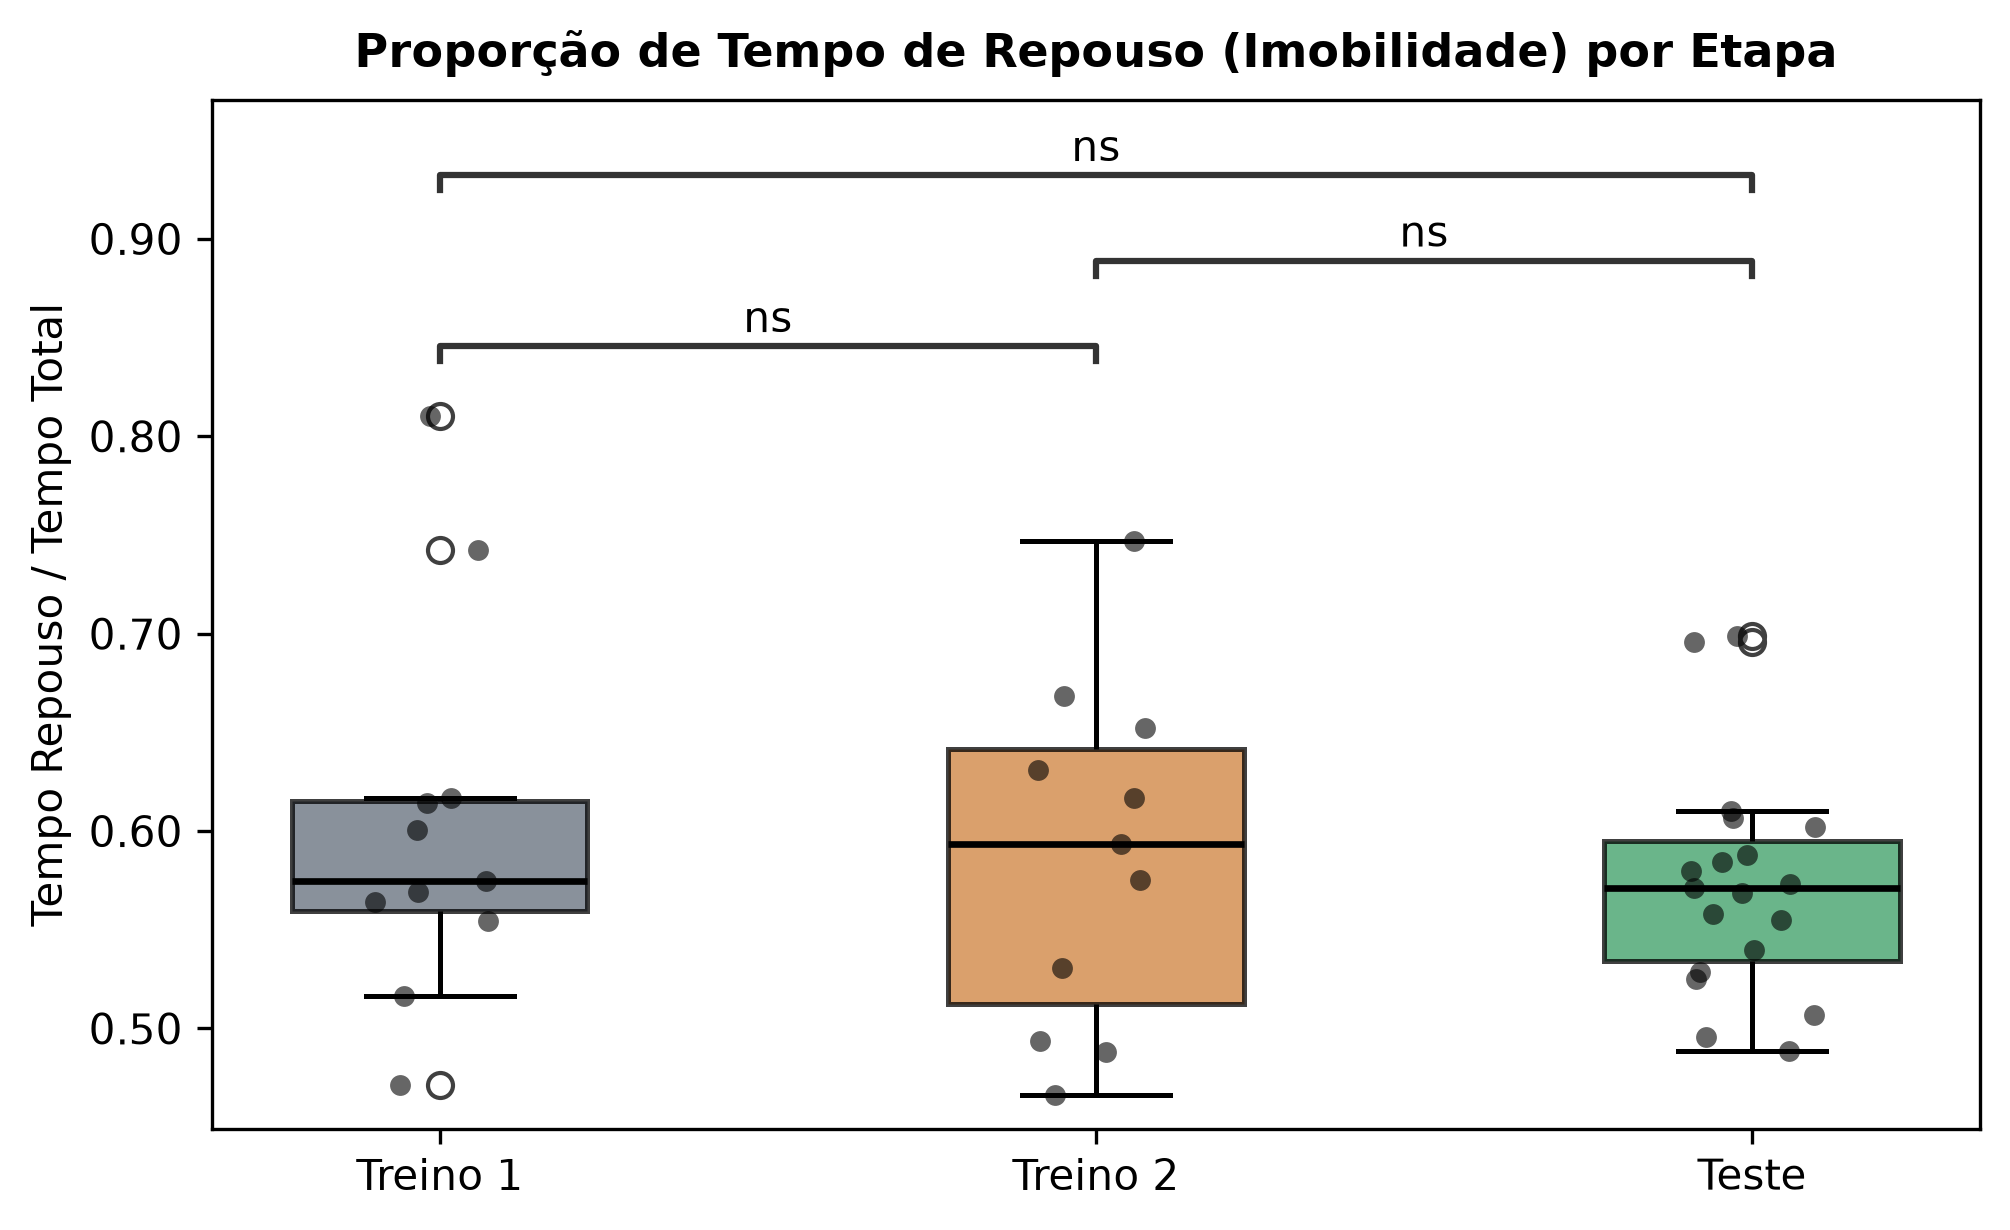
\includegraphics[width=0.68\textwidth]{grafico_comportamento_etapas_repouso.png}
    \caption{Proporção de repouso motor ao longo das etapas sequenciais do protocolo (Treino~1, Treino~2 e Teste). Todas as comparações foram estatisticamente não significantes (ns).}
    \label{fig:etapas_repouso}
\end{figure}

\begin{table}[tbp]
    \centering
    \small
    \setlength{\tabcolsep}{4.5pt}
    \caption{Parâmetros de mobilidade motora e atividade geral ao longo das etapas sequenciais do protocolo comportamental.}
    \label{tab:estatistica_etapas_movimento}
    \begin{adjustbox}{max width=0.95\textwidth}
        \begin{tabular}{lcccc}
            \toprule
            \textbf{Etapa} & \textbf{Sessões ($N$)} & \textbf{Exploração ($t_{\text{exp}}/t_{\text{tot}}$)} & \textbf{Repouso ($t_{\text{rep}}/t_{\text{tot}}$)} & \textbf{Movimento ($t_{\text{mov}}/t_{\text{tot}}$)} \\
            \midrule
            Treino 1       & 11                     & $0{,}048 \pm 0{,}034$                                 & $0{,}603 \pm 0{,}097$                              & $0{,}348 \pm 0{,}088$                                \\
            Treino 2       & 11                     & $0{,}065 \pm 0{,}021$                                 & $0{,}588 \pm 0{,}087$                              & $0{,}347 \pm 0{,}078$                                \\
            Teste          & 19                     & $0{,}060 \pm 0{,}027$                                 & $0{,}572 \pm 0{,}057$                              & $0{,}368 \pm 0{,}055$                                \\
            \midrule
            \textbf{ANOVA} & 41                     & $F = 1{,}03$ ($p = 0{,}367$)                          & $F = 0{,}56$ ($p = 0{,}577$)                       & $F = 0{,}42$ ($p = 0{,}661$)                         \\
            \bottomrule
        \end{tabular}
    \end{adjustbox}
    \vspace{0.2em}
    \begin{minipage}{0.95\textwidth}
        \footnotesize \textbf{Nota:} Média $\pm$ desvio padrão. Graus de liberdade: $F(2, 38)$. Comparações bivariadas para exploração: Treino~1 vs. Treino~2 ($p = 0{,}196$); Treino~2 vs. Teste ($p = 0{,}634$); Treino~1 vs. Teste ($p = 0{,}307$).
    \end{minipage}
\end{table}


A análise longitudinal confirma a estabilidade da atividade exploratória e dos intervalos de repouso ao longo de todo o cronograma experimental. A invariância desses índices assegura que os animais preservaram o impulso investigativo sem extinção comportamental, garantindo que as respostas motoras registradas decorrem unicamente da interação experimental padronizada.

\chapter{Modelagem Computacional de Circuitos Hipocampais}

\section{Fundamentação Epistemológica e Limites da Modelagem Computacional}

Antes de introduzir formulações matemáticas ou resultados numéricos, é indispensável delimitar com rigor o papel epistemológico das simulações computacionais em neurociência. Modelos computacionais \emph{in silico} não constituem uma réplica idêntica nem um substituto da realidade biológica \emph{in vivo}; eles representam simplificações fenomênicas estruturadas da dinâmica de tecidos excitáveis \cite{dayan2001, gerstner2014}.

Em ensaios comportamentais com roedores, a observação macroscópica (como o tempo de exploração de objetos na arena aberta) aborda o sistema nervoso central essencialmente como uma ``caixa-preta''. Quando um protocolo experimental de estimulação elétrica em malha aberta não resulta em diferenciação comportamental detectável entre padrões temporais, a mensuração motora isolada é incapaz de apontar em qual ponto da cadeia biofísica o sinal foi atenuado. O objetivo da modelagem computacional desenvolvida neste trabalho não é comprovar por que um ensaio empírico falhou, tampouco substituir a validação experimental. Trata-se, estritamente, de uma ferramenta analítica auxiliar para formular e testar hipóteses sobre possíveis restrições de processamento de sinais, saturação de condutâncias e limites de transmissão temporal em redes recorrentes \cite{dayan2001, buzsaki2006}.

Para fins de registro e consolidação de aprendizado próprio em neurociências, a introdução detalhada aos mecanismos neurofisiológicos modelados (neurônios piramidais excitatórios, interneurônios inibitórios rápidos, inibição perissomática por \emph{shunting}, depressão sináptica de curto prazo e cinética fotoquímica de opsinas) foi estruturada em um apêndice didático ao final deste relatório (\cref{apendice:mecanismos_neurofisiologicos}, localizado imediatamente antes das referências bibliográficas).

\section{Justificativa Metodológica da Arquitetura Adotada}

A modelagem de redes neurais biológicas exige a seleção cuidadosa do nível de abstração biofísica \cite{dayan2001, gerstner2014}. Por um lado, modelos multicompartimentais detalhados baseados no formalismo clássico de Hodgkin-Huxley \cite{hodgkin1952} e implementados em simuladores como o \textsf{NEURON} descrevem geometrias dendríticas tridimensionais complexas e dezenas de condutâncias iônicas voltagem-dependentes ($\text{Na}^+$, $\text{K}^+$, $\text{Ca}^{2+}$, $I_h$). Embora de alto realismo morfológico, esses modelos demandam dezenas de parâmetros livres que não foram calibrados diretamente por registros de \emph{patch-clamp} no tecido hipocampal sob as condições deste projeto. Essa proliferação paramétrica gera indeterminação identifiável, além de acarretar custos numéricos que inviabilizam simulações de redes recorrentes ao longo de centenas de ciclos de estimulação.

Por outro lado, modelos baseados puramente em taxa de disparo (\emph{Rate Models}) tratam a atividade neuronal como uma variável escalar contínua representando a frequência média de disparos \cite{dayan2001}. Embora computacionalmente leves, esses modelos descartam a cronometria fina de cada potencial de ação discreto. Dado que o objetivo central desta investigação reside em contrastar padrões de estimulação estruturados em bins temporais estritos de $\qty{14}{\milli\second}$ dentro de ciclos teta de $\qty{140}{\milli\second}$, a perda de resolução temporal intrínseca aos modelos de taxa impossibilitaria a discriminação dos intervalos inter-pulso.

Como compromisso analítico, adotou-se o modelo pontual bidimensional de Izhikevich \cite{izhikevich2003, izhikevich2007}. Esse modelo reduz a complexidade de bifurcação de Hodgkin-Huxley a um sistema diferencial de duas variáveis com regra de reinicialização descontínua, combinando a parcimônia computacional de modelos de integração e disparo (\emph{Integrate-and-Fire}) com a versatilidade biofísica de reproduzir a dinâmica rica de neurônios piramidais (adaptação lenta de frequência, RS) e interneurônios inibitórios locais (disparo rápido sem adaptação, FS).

Para contemplar o efeito cumulativo de sequências repetitivas de pulsos, o circuito incorpora a dinâmica sináptica de curto prazo descrita por Tsodyks e Markram \cite{tsodyks1997, tsodyks1998}, capturando a saturação do reservatório vesicular pré-sináptico. Ademais, inclui-se a população de interneurônios $\text{PV}^+$ responsáveis pelo shunting perissomático \cite{buzsaki2006}, permitindo avaliar como a inespecificidade do estímulo elétrico extracelular afeta o balanço excitação-inibição.

As simulações foram executadas no ambiente \textsf{Brian~2} \cite{stimberg2019}, um simulador de código aberto em Python projetado especificamente para redes de neurônios de disparo. A plataforma compila as equações diferenciais explicitadas pelo usuário em tempo de execução para código C/NumPy altamente vetorizado, garantindo verificação estrita de consistência dimensional em todas as variáveis de estado ($\unit{\milli\volt}$, $\unit{\milli\second}$, $\unit{\pico\farad}$, $\unit{\siemens}$) e reprodutibilidade numérica rigorosa.

\subsection{Parâmetros Biofísicos Calibrados e Proveniência Experimental}
\label{sec:parametros_biofisicos}
Para assegurar legibilidade integral e evitar perda de detalhes por redução de escala visual de tabelas, todos os parâmetros biofísicos empregados foram extraídos diretamente de literatura primária revisada por pares:
\begin{itemize}
    \item \textbf{Neurônios Piramidais de CA3 (Regular Spiking -- RS):}
          \begin{itemize}
              \item Escala temporal de recuperação da variável lenta: $a = 0{,}02$ \cite{izhikevich2003}.
              \item Sensibilidade sub-limiar de $u$ em relação a flutuações de $v$: $b = 0{,}20$ \cite{izhikevich2003}.
              \item Potencial de repolarização pós-disparo: $c = \qty{-65}{\milli\volt}$, correspondendo ao potencial de repouso fisiológico \cite{izhikevich2003}.
              \item Incremento de adaptação pós-disparo: $d = \qty{8}{\milli\volt}$, reproduzindo a adaptação de frequência gradual de células piramidais corticais e hipocampais \cite{izhikevich2003}.
          \end{itemize}
    \item \textbf{Interneurônios Inibitórios Locais \texorpdfstring{$\text{PV}^+$}{PV+} (Fast Spiking -- FS):}
          \begin{itemize}
              \item Escala temporal de recuperação: $a = 0{,}10$, conferindo restauração ultrarrápida do estado basal \cite{izhikevich2003}.
              \item Sensibilidade sub-limiar: $b = 0{,}20$ \cite{izhikevich2003}.
              \item Potencial de repolarização pós-disparo: $c = \qty{-65}{\milli\volt}$ \cite{izhikevich2003}.
              \item Incremento de adaptação: $d = \qty{2}{\milli\volt}$, permitindo sustentar frequências $> \qty{150}{\hertz}$ sem decaimento de taxa \cite{izhikevich2003}.
          \end{itemize}
    \item \textbf{Dinâmica Sináptica de Curto Prazo (Tsodyks-Markram):}
          \begin{itemize}
              \item Tempo de reciclagem e ancoragem vesicular: $\tau_{\text{rec}} = \qty{600}{\milli\second}$, medido experimentalmente em fatias de hipocampo \cite{tsodyks1998}.
              \item Fração de liberação por evento pré-sináptico: $U = 0{,}45$, refletindo a probabilidade de exocitose vesicular basal \cite{tsodyks1998}.
              \item Constante de decaimento inibitório perissomático mediado por cloreto: $\tau_{\text{GABA}} = \qty{6}{\milli\second}$, com potencial de reversão $E_{\text{GABA}} = \qty{-75}{\milli\volt}$.
          \end{itemize}
    \item \textbf{Cinética de Opsinas Microbianas (Transdução Óptica):}
          \begin{itemize}
              \item Taxa de ativação fotônica sob irradiação de laser azul ($\qty{488}{\nano\meter}$): $\alpha = \qty{0{,}8}{\per\milli\second}$ \cite{grossman2011}.
              \item Tempo de desativação espontânea da Canalrodopsina-2 clássica (ChR2 wild-type): $\tau_{\text{off}} = \qty{13{,}0}{\milli\second}$, estabelecido por medições de \emph{patch-clamp} em células de mamíferos a temperatura ambiente ($\qty{10}{\milli\second}$ a $\qty{13}{\milli\second}$) \cite{nagel2003, grossman2011}.
              \item Tempo de desativação espontânea da opsina  Chronos: $\tau_{\text{off}} = \qty{3{,}6}{\milli\second}$, caracterizado em \emph{whole-cell patch-clamp} a $\qty{22}{\degreeCelsius}$ ($3{,}6 \pm 0{,}2\ \unit{\milli\second}$) isolada de \emph{Stigeoclonium helveticum} por Klapoetke et al. \cite{klapoetke2014}.
          \end{itemize}
\end{itemize}

\section{Formulação Matemática dos Componentes Biofísicos}

\subsection{Dinâmica dos Neurônios Piramidais Excitatórios (RS)}
Os neurônios piramidais foram modelados segundo o sistema bidimensional de Izhikevich \cite{izhikevich2003}:
\begin{align}
    \frac{\mathrm{d}v}{\mathrm{d}t} & = \frac{0{,}04\,v^2 + 5\,v + 140 - u + I_{\text{ext}} + I_{\text{syn\_exc}} - I_{\text{syn\_inh}}}{C_m} \\[0.5em]
    \frac{\mathrm{d}u}{\mathrm{d}t} & = a\,(b\,v - u)
\end{align}
com reinicialização descontínua de limiar:
\begin{equation}
    \text{se } v \ge \qty{30}{\milli\volt}, \quad \text{então } \begin{cases} v \leftarrow c \\ u \leftarrow u + d \end{cases}
\end{equation}
onde $v$ é o potencial transmembrana ($\unit{\milli\volt}$), $u$ é a variável de recuperação lenta, $a = 0{,}02$ define a taxa temporal de recuperação, $b = 0{,}20$ dita a sensibilidade de $u$ às oscilações sub-limiares de $v$, $c = \qty{-65}{\milli\volt}$ é o potencial de repolarização pós-disparo e $d = \qty{8}{\milli\volt}$ é o incremento de adaptação por disparo (conforme detalhado na \cref{sec:parametros_biofisicos}).

\subsection{Dinâmica dos Interneurônios Inibitórios \texorpdfstring{$\text{PV}^+$}{PV+} (FS)}
Os interneurônios inibitórios locais foram modelados com cinética de disparo rápido (\emph{Fast Spiking}):
\begin{equation}
    a = 0{,}10, \quad b = 0{,}20, \quad c = \qty{-65}{\milli\volt}, \quad d = \qty{2}{\milli\volt}
\end{equation}
Essa parametrização confere baixa reobase, rápida restauração do estado inicial e ausência de acúmulo de adaptação, viabilizando disparos contínuos em frequências elevadas sob excitação extracelular direta.

\subsection{Inibição Perissomática por Shunting}
A corrente inibitória pós-sináptica mediada por receptores $\text{GABA}_A$ perissomáticos é descrita por:
\begin{equation}
    I_{\text{syn\_inh}} = g_{\text{GABA}}(t)\,(v - E_{\text{GABA}})
\end{equation}
com condutância de decaimento exponencial ($\tau_{\text{GABA}} = \qty{6}{\milli\second}$) e potencial de reversão $E_{\text{GABA}} = \qty{-75}{\milli\volt}$. Dada a proximidade de $E_{\text{GABA}}$ ao potencial de repouso, a condutância atua preponderantemente reduzindo a resistência efetiva de entrada da célula, drenando correntes despolarizantes incidentes.

\subsection{Dinâmica Sináptica de Depleção Vesicular (Tsodyks-Markram)}
A depressão de curto prazo nas sinapses excitatórias recorrentes segue o modelo de Tsodyks-Markram \cite{tsodyks1998}:
\begin{equation}
    \frac{\mathrm{d}R}{\mathrm{d}t} = \frac{1 - R}{\tau_{\text{rec}}} - U\,R\,\sum_{k} \delta(t - t_k)
\end{equation}
onde $R(t) \in [0, 1]$ denota a fração de vesículas disponíveis no reservatório prontamente liberável, $\tau_{\text{rec}} = \qty{600}{\milli\second}$ é a constante temporal de reciclagem e ancoragem vesicular, e $U = 0{,}45$ é a fração esgotada a cada potencial de ação pré-sináptico no instante $t_k$.

\subsection{Cinética de Fotoestimulação por Opsinas Microbianas}
A transdução optogenética foi expressa pelo modelo fotoquímico de dois estados \cite{nikolic2009, grossman2011}:
\begin{equation}
    \frac{\mathrm{d}O}{\mathrm{d}t} = \alpha\,L(t)\,(1 - O) - \frac{O}{\tau_{\text{off}}}
\end{equation}
onde $O(t) \in [0, 1]$ é a fração de canais abertos, $L(t) \in \{0, 1\}$ é o estado do pulso óptico, $\alpha = \qty{0{,}8}{\per\milli\second}$ é a taxa de fotoativação e $\tau_{\text{off}}$ é a constante de desativação espontânea ao escuro ($\qty{13{,}0}{\milli\second}$ para ChR2 e $\qty{3{,}6}{\milli\second}$ para Chronos; conforme detalhado na \cref{sec:parametros_biofisicos}).

\subsection{Métrica de Correlação Temporal de Disparo por Bin (Correlação de Pearson)}
Para quantificar se os neurônios diferenciam os dois padrões no domínio do tempo além da mera contagem agregada de eventos, discretizou-se o ciclo teta ($\qty{140}{\milli\second}$) nos mesmos 10 bins de $\qty{14}{\milli\second}$ do protocolo experimental, computando o Perfil Temporal Médio de Disparo (\emph{Peri-Stimulus Time Histogram} -- PSTH) da população:
\begin{equation}
    \mathbf{p} = [p_1, p_2, \dots, p_{10}]^T
\end{equation}
onde $p_k$ representa a contagem acumulada de disparos emitidos pelos neurônios no $k$-ésimo bin do ciclo. A similaridade na modulação de fase temporal entre os padrões $S_1$ e $S_2$ é quantificada diretamente pelo coeficiente de correlação linear de Pearson ($r$):
\begin{equation}
    r(\mathbf{p}_{S_1}, \mathbf{p}_{S_2}) = \frac{\sum_{k=1}^{10} (p_{S_1, k} - \bar{p}_{S_1})(p_{S_2, k} - \bar{p}_{S_2})}{\sqrt{\sum_{k=1}^{10} (p_{S_1, k} - \bar{p}_{S_1})^2} \sqrt{\sum_{k=1}^{10} (p_{S_2, k} - \bar{p}_{S_2})^2}}
\end{equation}
Valores de $r \approx 1$ indicam que as populações disparam sincronizadas nos mesmos bins temporais (formas de onda de disparo idênticas), ao passo que $r \approx 0$ ou $r < 0$ comprovam que os disparos ocorrem em fases descorrelacionadas ou alternadas ao longo do ciclo teta.

\subsection{Avaliação Estatística: Teste de Equivalência Biológica (TOST) e Limites do Teste t em Simulações}
A avaliação inferencial de modelos computacionais em neurociência impõe um desafio epistemológico que difere dos ensaios de bancada com animais vivos. Em simulações com população finita ($N = 80$ células) descritas por equações diferenciais sob baixo ruído de condutância, o erro padrão da média ($SE = s / \sqrt{N}$) é muito reduzido. Sob essas condições, o teste $t$ de Student convencional de hipótese nula pontual ($H_0: \mu_1 - \mu_2 = 0$) incorre na chamada falácia do superpoder amostral ou paradoxo de baixo ruído (\emph{large-sample / low-noise fallacy}) \cite{lakens2017}: qualquer flutuação microscópica estritamente matemática (como uma variação média de apenas 2 disparos ao longo de mais de um segundo) adquire significância estatística espúria ($p < 0{,}001$), gerando uma aparente contradição entre significância estatística e irrelevância biológica real. Adicionalmente, contagens de disparos constituem dados inteiros discretos; o teste de Shapiro-Wilk sobre as diferenças célula a célula confirma desvio da normalidade ($W = 0{,}890$, $p = 4{,}76 \times 10^{-6}$), violando a premissa de distribuição gaussiana contínua do teste $t$ paramétrico.

Para superar essa limitação e determinar se as taxas de disparo são de fato biologicamente equivalentes na prática, utilizou-se o \textbf{Teste de Equivalência por Duas Hipóteses Unilaterais} (\emph{Two One-Sided Tests} -- TOST) \cite{schuirmann1987, lakens2017}. No procedimento TOST, define-se a priori uma Margem de Equivalência Biológica ($\Delta_B$), ancorada na variabilidade basal de condutâncias e taxas de disparo espontâneas em circuitos hipocampais vivos ($10\%$ a $15\%$ da taxa basal, isto é, $\Delta_B = \pm 5{,}69$ disparos) \cite{buzsaki2006, gerstner2014}. O teste avalia simultaneamente duas hipóteses unilaterais:
\begin{align}
    H_{01}: \mu_{S_1} - \mu_{S_2} \le -\Delta_B \quad & \text{vs} \quad H_{11}: \mu_{S_1} - \mu_{S_2} > -\Delta_B \\
    H_{02}: \mu_{S_1} - \mu_{S_2} \ge +\Delta_B \quad & \text{vs} \quad H_{12}: \mu_{S_1} - \mu_{S_2} < +\Delta_B
\end{align}
O valor-$p$ consolidado do TOST é dado pelo máximo entre as duas estatísticas: $p_{\text{TOST}} = \max(p_1, p_2)$. Caso $p_{\text{TOST}} < 0{,}05$, rejeita-se a presença de qualquer efeito que atinja relevância fisiológica e conclui-se formalmente que \textbf{as taxas de disparo são estatisticamente equivalentes entre si}.

\section{Escala Populacional dos Microcircuitos}
\label{sec:escala_rede_parcimonia}

Uma decisão metodológica central na modelagem de sistemas neurais reside na definição da escala populacional e na justificativa epistemológica de sua dimensionalidade. No presente trabalho, dois desenhos populacionais distintos foram empregados no ambiente \textsf{Brian~2}:
\begin{enumerate}
    \item \textbf{Experimento 1 (Estimulação Elétrica Extracelular):} rede de microcircuito recorrente contendo exatamente $N = 100$ neurônios ($80$ células piramidais excitatórias e $20$ interneurônios inibitórios locais).
    \item \textbf{Experimento 2 (Optogenética):} modelo de $1$ neurônio piramidal representativo infectado por opsinas, simulado ao longo de 10 ciclos teta consecutivos.
\end{enumerate}

Essa diferenciação não é acidental; ela decorre estritamente da pergunta formulada para cada ensaio e do princípio da parcimônia biofísica, conforme justificado a seguir.

\subsection{A Proporção 80/20 e o Microcircuito Mínimo no Experimento 1}
A adoção de 80 neurônios piramidais (RS) e 20 interneurônios inibitórios (FS) no Experimento 1 não constitui uma escolha arbitrária, mas reflete a \textbf{proporção citoarquitetônica canônica} documentada na neuroanatomia quantitativa do hipocampo e do neocórtex de roedores \cite{buzsaki2006, kandel2021}. Em subcampos hipocampais como CA3 e CA1, aproximadamente $80\%$ das células neuronais são neurônios de projeção excitatórios glutamatérgicos (células piramidais), enquanto os $20\%$ remanescentes compreendem uma população heterogênea de interneurônios inibitórios GABAérgicos locais, dominada funcionalmente por células em cesto imunorreativas à parvalbumina ($\text{PV}^+$) \cite{buzsaki2006}.

Em termos de escala computacional, $100$ neurônios representam o \textbf{microcircuito canônico mínimo} (\emph{canonical microcircuit}) capaz de instanciar formalmente as interações essenciais de uma microcoluna:
\begin{itemize}
    \item Excitação recorrente entre células piramidais ($E \to E$, mediada por receptores AMPA);
    \item Recrutamento excitatório de interneurônios inibitórios por aferências piramidais ($E \to I$);
    \item Inibição perissomática por retroalimentação (\emph{feedback inhibition}) e por antecipação (\emph{feedforward shunting}, $I \to E$, mediada por $\text{GABA}_A$).
\end{itemize}

\subsection{Capacidade Explicativa versus Limites Biológicos}
O subcampo CA3 de um camundongo adulto abriga cerca de $300.000$ neurônios. Diante dessa disparidade de escala, é epistemologicamente indispensável delimitar com clareza o que a rede de 100 neurônios é capaz de explicar e o que ela deliberadamente não se propõe a representar:
\begin{itemize}
    \item \textbf{O que o modelo não representa:} A simulação de 100 células não reproduz a dinâmica cognitiva global de um animal livre em arena física, não contempla a geometria tridimensional do tecido ou o decaimento espacial do campo elétrico ($1/r^2$) em relação à ponta do microeletrodo metálico, e não modela a alça polissináptica completa entre CA3, CA1 e o córtex entorrinal.
    \item \textbf{O que o modelo explica:} O mérito do modelo não reside em predizer escolhas motoras macroscópicas, mas em isolar \textbf{mecanismos biofísicos locais de processamento de sinais} que operam no nível da membrana e da fenda sináptica:
          \begin{enumerate}
              \item \emph{Saturação e esgotamento vesicular:} a dinâmica de depleção de Tsodyks-Markram opera no terminal pré-sináptico individual. O colapso do reservatório de vesículas prontamente liberáveis ($R(t) \approx 0{,}11$) sob estimulação contínua a $\qty{8}{\hertz}$ em malha aberta independe de a rede possuir 100 ou 300 mil células; trata-se de uma propriedade biofísica da fenda sináptica.
              \item \emph{Curto-circuito por inibição (\emph{shunting}):} o microeletrodo metálico extracelular não possui seletividade molecular, despolarizando fibras sem distinção celular. Em virtude de sua menor reobase, os interneurônios $\text{PV}^+$ disparam prontamente, acionando um divisor resistivo que silencia as piramidais. Esse fenômeno é capturado de forma fidedigna no microcircuito de 100 células.
              \item \emph{Desfasamento temporal em fase teta:} permite testar formalmente se a alternância microscópica de pulsos em bins de $\qty{14}{\milli\second}$ preserva resolução temporal ($r < 0$ no PSTH) ou se é mascarada pela taxa média agregada ($p_{\text{TOST}} < 0{,}05$).
          \end{enumerate}
\end{itemize}

\subsection{Isolamento de Célula Representativa no Experimento 2}
Em contrapartida ao Experimento 1, o Experimento 2 (baseado no protocolo de Costa \cite{costa2026}) utilizou um modelo de \textbf{1 neurônio piramidal representativo} (\texttt{NeuronGroup(1)} avaliado em 10 ciclos teta). Essa escolha reflete duas particularidades biológicas fundamentais:
\begin{enumerate}
    \item \textbf{Seletividade Genética Celular:} O protocolo optogenético utilizou vetores virais adenoassociados (AAV) com promotor específico $\alpha$-CaMKII, restringindo a expressão de ChR2 exclusivamente a neurônios piramidais excitatórios de CA3 e poupando completamente os interneurônios inibitórios GABAérgicos. Logo, não havia recrutamento sináptico inespecífico do freio inibitório perissomático via $\text{PV}^+$.
    \item \textbf{Gargalo Biofísico de Canal versus Conectividade de Rede:} A investigação empírica de Costa \cite{costa2026} visava explicar por que dois padrões ópticos com mesma dose total de energia ($MS_f$ versus $MS_r$) não produziram separação na expressão histológica da proteína c-Fos ($p = 0{,}9888$). A questão biofísica central não residia na topologia sináptica da rede, mas na \textbf{cinética fotoquímica intrínseca de abertura e fechamento do poro da opsina} ($\tau_{\text{off}} = \qty{13{,}0}{\milli\second}$ em ChR2 versus $\qty{3{,}6}{\milli\second}$ em Chronos) e no consequente influxo cumulativo de cálcio intracelular $[\text{Ca}^{2+}](t)$, sinalizador proximal da transcrição gênica de c-Fos.
\end{enumerate}
Sob iluminação focal uniforme por laser azul ($\qty{488}{\nano\meter}$), todas as células piramidais infectadas obedecem rigorosamente às mesmas equações diferenciais fotoquímicas de transição de estado. Portanto, simular uma população de centenas de neurônios desacoplados sinapticamente geraria cópias idênticas da mesma dinâmica média. O isolamento de uma célula piramidal representativa atende plenamente ao princípio da parcimônia metodológica, reduzindo o modelo às variáveis que governam o fenômeno sob escrutínio.

\section{Experimento 1: Microestimulação Elétrica Extracelular em CA3}

O primeiro experimento computacional avaliou a resposta de um microcircuito hipocampal canônico contendo 80 neurônios piramidais (RS) e 20 interneurônios inibitórios $\text{PV}^+$ (FS), totalizando 100 células estruturadas na proporção canônica 80/20 (\cref{sec:escala_rede_parcimonia}), interconectadas por condutâncias recorrentes AMPA e $\text{GABA}_A$, sob estimulação elétrica bifásica ($\qty{25}{\micro\ampere}$, $\qty{100}{\micro\second}$ por fase) em coordenadas estereotáxicas de CA3 ventral (AP: $-3{,}30\ \text{mm}$; ML: $\pm 2{,}50\ \text{mm}$; DV: $-4{,}00\ \text{mm}$).

Comparou-se a resposta do circuito a dois padrões temporais em ciclos teta de $\qty{140}{\milli\second}$ divididos em bins de $\qty{14}{\milli\second}$: o Padrão 1 ($S_1$: \texttt{1010101101}, 6 pulsos ativos por ciclo) e o Padrão 2 ($S_2$: \texttt{1110010111}, 7 pulsos ativos por ciclo), sob regime contínuo de malha aberta simulando a sessão experimental executada na bancada (\cref{fig:exp1_eletrica}).

\subsection{Definição das Hipóteses Estatísticas}
\begin{itemize}
    \item \textbf{Hipótese Nula de Taxa Escalar (Equivalência Biológica via TOST):} A diferença na taxa média de disparos entre $S_1$ e $S_2$ situa-se estritamente dentro da margem de equivalência biológica de $15\%$ ($H_0: |\mu_{S_1} - \mu_{S_2}| < \Delta_B$).
    \item \textbf{Hipótese Nula de Código Temporal (Correlação de Pearson no PSTH):} Os perfis temporais de disparo por bin são correlacionados ao longo do ciclo teta ($H_0: r \approx 1$).
    \item \textbf{Hipótese Alternativa de Código Temporal ($H_1$):} Os padrões produzem desfasamento temporal estrito ao longo dos bins do ciclo teta ($H_1: r \ll 1$ ou $r < 0$).
\end{itemize}

\begin{figure}[!ht]
    \centering
    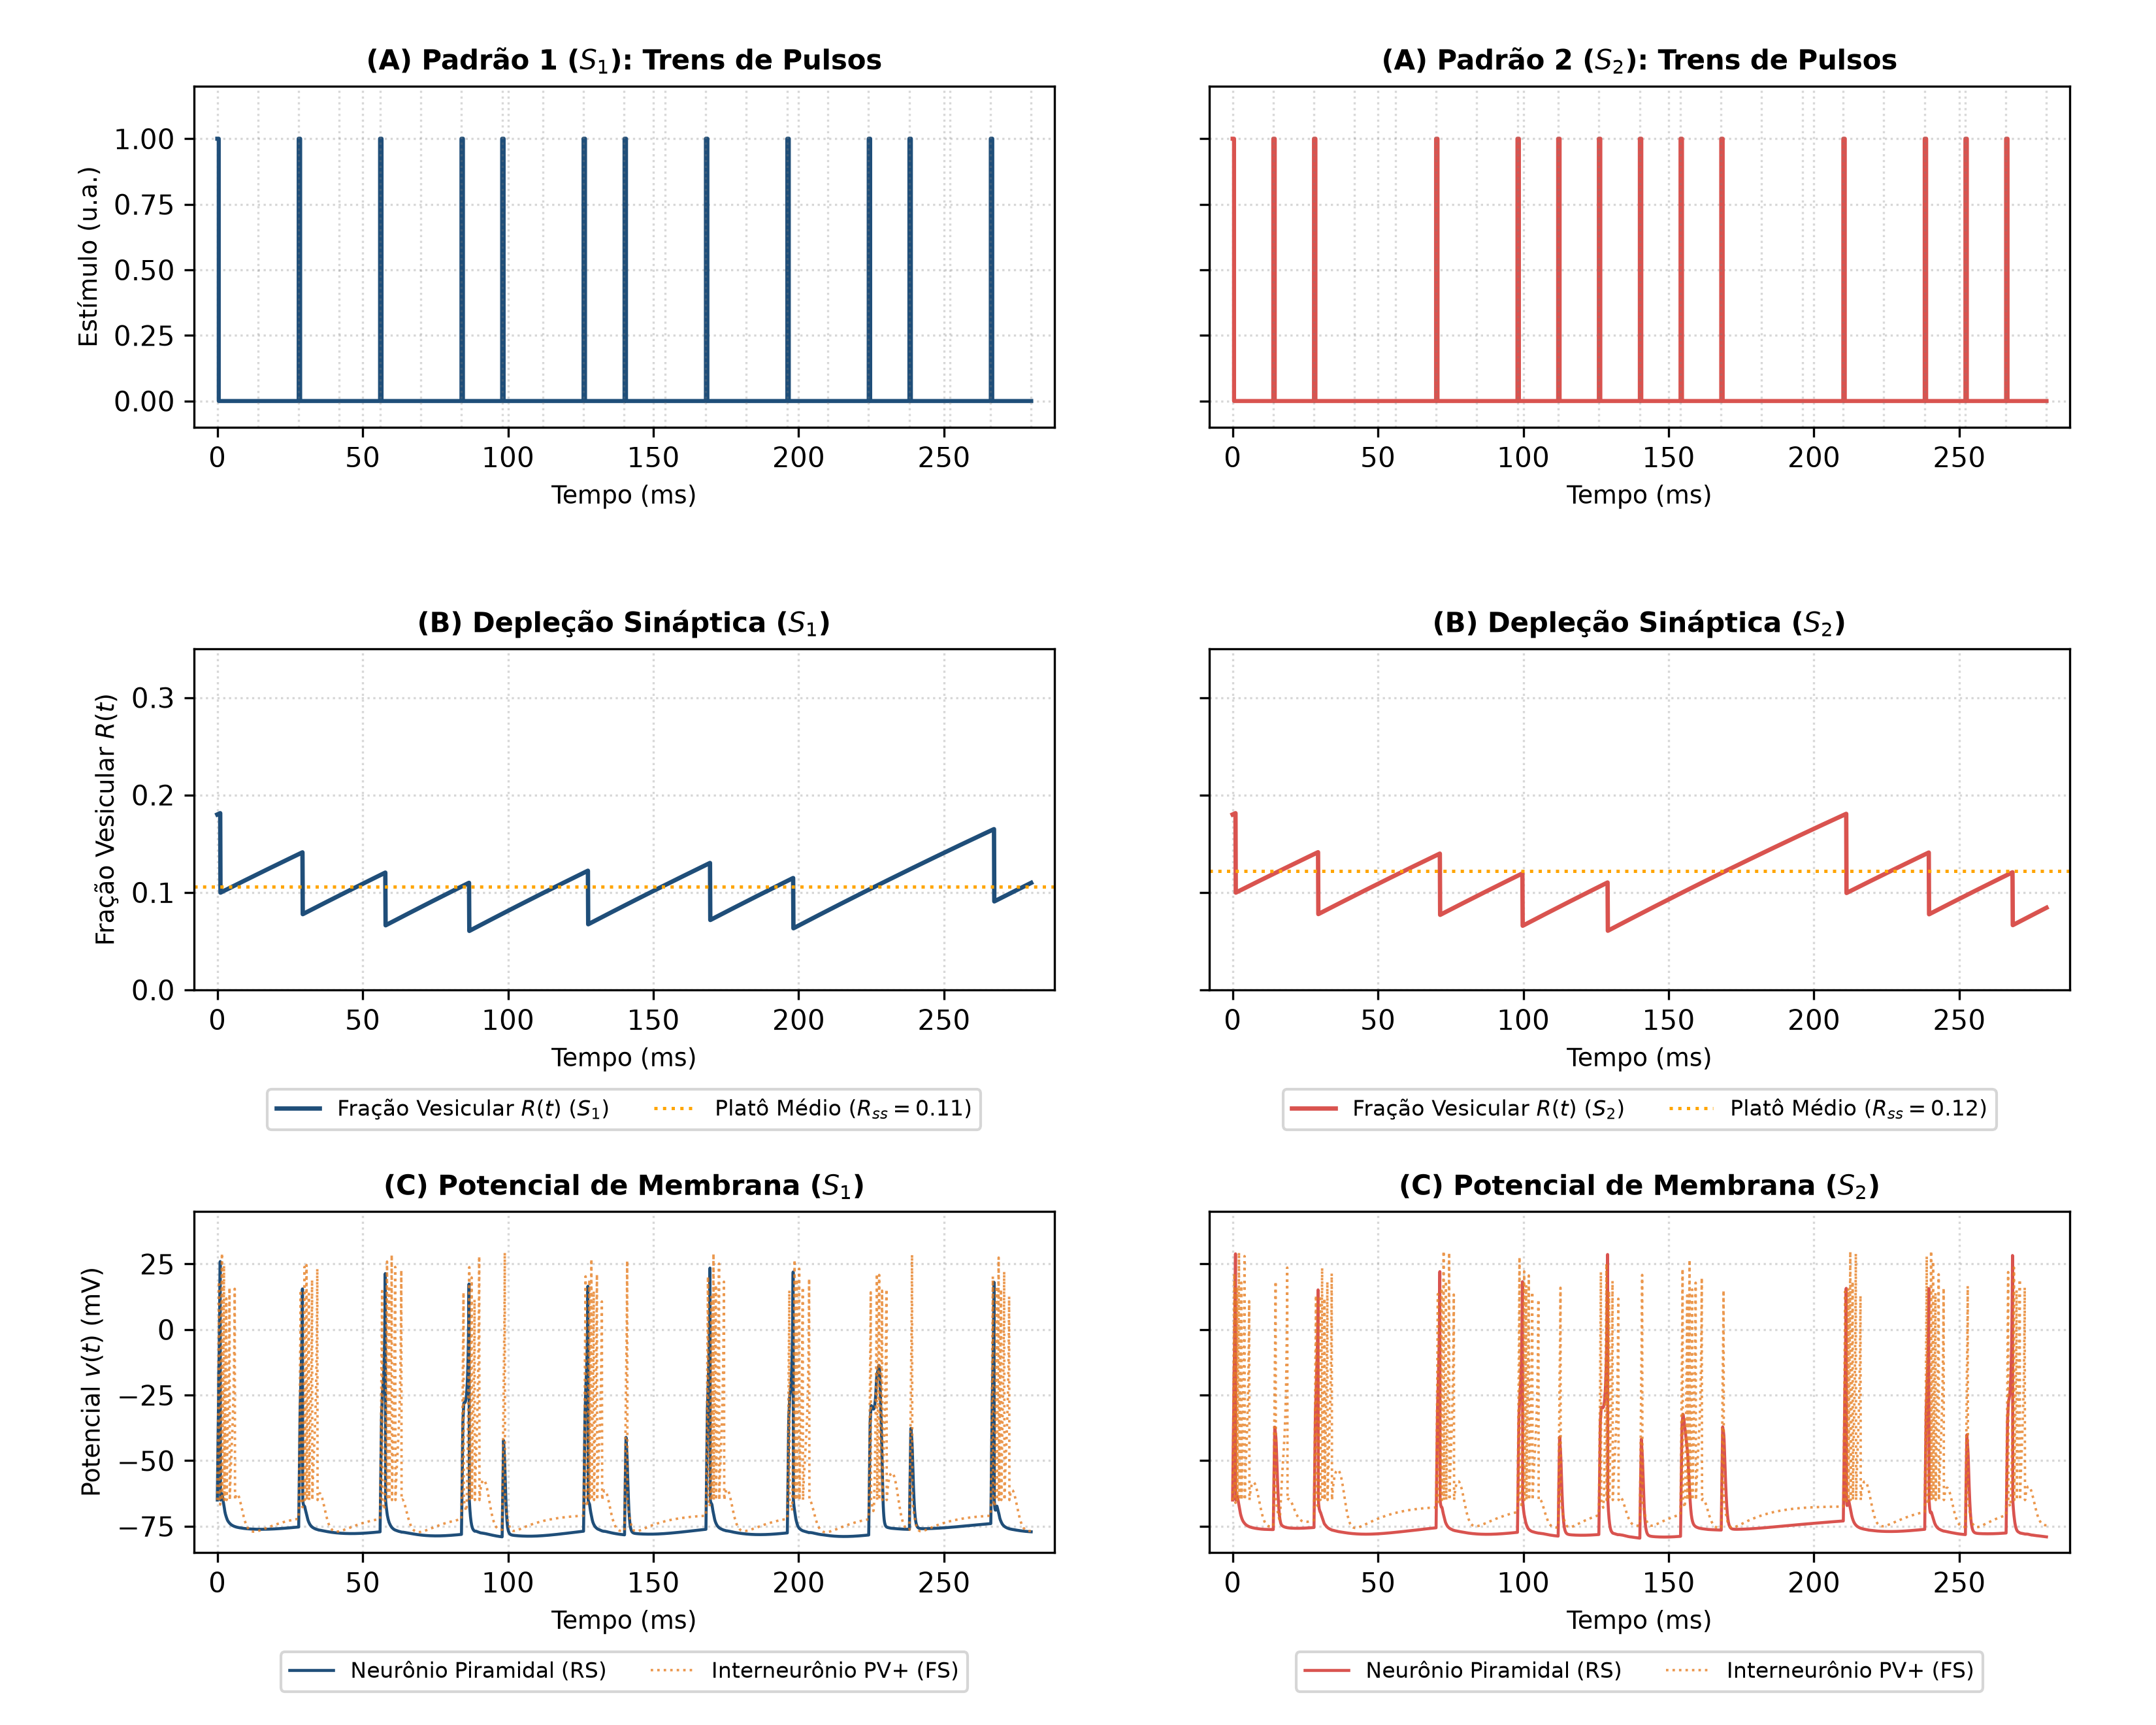
\includegraphics[width=0.98\textwidth]{experimento_1_eletrica_wagner_brian2.png}
    \caption[Simulação em Brian 2 da microestimulação elétrica extracelular]{Simulação em \textsf{Brian~2} da microestimulação elétrica extracelular contínua em microcircuito de CA3. Disposição em duas colunas com eixos compartilhados por linha para comparação direta entre o Padrão 1 ($S_1$; coluna esquerda) e o Padrão 2 ($S_2$; coluna direita). (A) Trens de pulsos elétricos aplicados nos bins de $\qty{14}{\milli\second}$ do ciclo teta ($\qty{140}{\milli\second}$). (B) Dinâmica da fração de vesículas disponíveis $R(t)$ pelo modelo de Tsodyks-Markram ($\tau_{\text{rec}} = \qty{600}{\milli\second}$, $U = 0{,}45$). (C) Potencial transmembrana $v(t)$ de neurônios piramidais (RS, traço azul) e interneurônios inibitórios $\text{PV}^+$ (FS, traço vermelho).}
    \label{fig:exp1_eletrica}
\end{figure}

\begin{table}[tbp]
    \centering
    \small
    \setlength{\tabcolsep}{3.5pt}
    \caption{Quantificação de disparos e teste de equivalência biológica (TOST) na população de CA3 no Experimento 1.}
    \label{tab:resultados_exp1_disparos}
    \begin{tabular}{lcccc}
        \toprule
        \textbf{Padrão} & \textbf{Pulsos/Ciclo} & \textbf{Disparos Totais} & \textbf{Disparos / Célula} & \textbf{Taxa Média Pop.} \\
        \midrule
        Padrão 1 ($S_1$) & 6 & $3.037$ & $37{,}96 \pm 4{,}53$ & \qty{27{,}12}{\hertz} $\pm$ \qty{3{,}24}{\hertz} \\
        Padrão 2 ($S_2$) & 7 & $2.852$ & $35{,}65 \pm 4{,}80$ & \qty{25{,}46}{\hertz} $\pm$ \qty{3{,}43}{\hertz} \\
        \midrule
        \textbf{Comparação} & $+16{,}7\%$ & $\Delta = 6{,}09\%$ & \multicolumn{2}{c}{TOST ($15\%$): $t_2 = -5{,}22;\ p_{\text{TOST}} < 10^{-6}$} \\
        \bottomrule
    \end{tabular}
    \vspace{0.2em}
    \begin{minipage}{0.95\textwidth}
        \footnotesize \textbf{Nota:} Quantificação sobre $N=80$ neurônios piramidais em 10 ciclos teta ($\qty{1{,}4}{\second}$). A equivalência prática foi avaliada pelo procedimento TOST (\emph{Two One-Sided Tests}) com margem fisiológica de $\pm 15\%$ ($\pm 5{,}69$ disparos), comprovando equivalência estatística estrita ($p_{\text{TOST}} < 0{,}001$; sob margem de $10\%$, $p_{\text{TOST}} = 0{,}0124$). O teste $t$ pontual convencional rejeitaria $H_0$ ($t(79) = 3{,}568, p = 0{,}00062$) em função do superpoder amostral de simulações com baixo ruído, contrastando com a equivalência biológica real.
    \end{minipage}
\end{table}

\begin{table}[tbp]
    \centering
    \footnotesize
    \setlength{\tabcolsep}{3pt}
    \caption{Dinâmica de depleção vesicular e correlação temporal de disparo no Experimento 1.}
    \label{tab:resultados_exp1_dinamica}
    \begin{tabular}{lcccc}
        \toprule
        \textbf{Padrão} & \textbf{$R_{\text{ss}}$} & \textbf{$R_{\text{mín}}$} & \textbf{Correlação Pop. ($r$)} & \textbf{Correlação Célula ($r$)} \\
        \midrule
        Padrão 1 ($S_1$) & $0{,}1058$ & $0{,}0605$ & \multirow{2}{*}{$r = -0{,}3035$} & \multirow{2}{*}{$-0{,}2705 \pm 0{,}1794$} \\
        Padrão 2 ($S_2$) & $0{,}1223$ & $0{,}0607$ & & \\
        \midrule
        \textbf{Regime} & \multicolumn{2}{c}{Depleção estacionária ($\approx 89\%$)} & \multicolumn{2}{c}{\textbf{Defasagem temporal estrita ($r < 0$)}} \\
        \bottomrule
    \end{tabular}
    \vspace{0.2em}
    \begin{minipage}{0.95\textwidth}
        \footnotesize \textbf{Nota:} $R_{\text{ss}}$ e $R_{\text{mín}}$ representam a fração vesicular estacionária média e mínima de Tsodyks-Markram ($\tau_{\text{rec}} = \qty{600}{\milli\second}$, $U = 0{,}45$). A correlação linear de Pearson ($r$) foi calculada sobre os perfis temporais médios de disparo (PSTH com 10 bins de $\qty{14}{\milli\second}$ do ciclo teta de $\qty{140}{\milli\second}$), comprovando que os disparos ocorrem em fases descorrelacionadas entre $S_1$ e $S_2$.
    \end{minipage}
\end{table}


\subsection{Análise da Dinâmica Sináptica e Avaliação por Métricas Temporais}
Os dados quantitativos extraídos da simulação computacional (\cref{fig:exp1_eletrica} e \cref{tab:resultados_exp1_disparos,tab:resultados_exp1_dinamica}) elucidam o processamento do estímulo elétrico contínuo no microcircuito:
\begin{enumerate}
    \item \textbf{Depleção Vesicular Sustentada de Tsodyks-Markram:} Sob estimulação contínua, a fração de vesículas disponíveis $R(t)$ colapsa rapidamente nos primeiros pulsos e opera em patamar estacionário severamente deprimido: $R_{\text{ss}} = 0{,}1058$ ($R_{\text{mín}} = 0{,}0605$, $\text{Var} = 0{,}00053$) para o Padrão 1, e $R_{\text{ss}} = 0{,}1223$ ($R_{\text{mín}} = 0{,}0607$, $\text{Var} = 0{,}00088$) para o Padrão 2. Como a constante de reciclagem vesicular ($\tau_{\text{rec}} = \qty{600}{\milli\second}$) é muito superior aos intervalos inter-pulso ($\qty{14}{\milli\second}$ a $\qty{28}{\milli\second}$), $R(t)$ \textbf{não retorna a valores elevados durante toda a estimulação}. As sinapses recorrentes permanecem atenuadas, desacoplando o feedback excitatório na rede.
    \item \textbf{Recrutamento Inespecífico e Shunting Inibitório:} O estímulo extracelular despolariza concomitantemente células piramidais e interneurônios $\text{PV}^+$. Em função de sua menor reobase, os interneurônios disparam de forma imediata e síncrona (\cref{fig:exp1_eletrica}C), acionando condutâncias $\text{GABA}_A$ perissomáticas que estabelecem um divisor resistivo para terra (\emph{shunting}), estreitando a janela de integração das células piramidais.
    \item \textbf{Equivalência Estatística de Taxa (TOST) versus Codificação Temporal (PSTH):} Sob a métrica escalar de contagem de disparos da população de 80 neurônios piramidais, obteve-se $37{,}96 \pm 4{,}53$ disparos/célula para $S_1$ ($\qty{27{,}12}{\hertz} \pm \qty{3{,}24}{\hertz}$) e $35{,}65 \pm 4{,}80$ disparos/célula para $S_2$ ($\qty{25{,}46}{\hertz} \pm \qty{3{,}43}{\hertz}$), totalizando $3.037$ versus $2.852$ potenciais de ação ($\Delta_{\text{taxa}} = 6{,}09\%$; diferença média de apenas $2{,}31$ disparos em $\qty{1{,}4}{\second}$; \cref{tab:resultados_exp1_disparos}). O teste de equivalência TOST com margem biológica de $15\%$ ($\Delta_B = \pm 5{,}69$ disparos) resultou em $t_1 = 12{,}36$ ($p_1 < 10^{-15}$) e $t_2 = -5{,}218$ ($p_2 = 7{,}12 \times 10^{-7}$), estabelecendo $p_{\text{TOST}} = 7{,}12 \times 10^{-7}$ ($p < 0{,}001$). Mesmo sob uma margem estrita de $10\%$ ($\Delta_B = \pm 3{,}80$ disparos), obtém-se $p_{\text{TOST}} = 0{,}0124$ ($p < 0{,}05$). Esse resultado comprova que \textbf{a taxa média agregada é formal e estatisticamente equivalente entre os padrões}, eliminando a distorção do teste $t$ pontual que acusaria significância espúria ($p = 0{,}00062$) em função do baixo ruído in silico. Em contrapartida, a avaliação temporal da forma de onda de disparos por bin (PSTH) revelou uma correlação linear de Pearson negativa: $r = -0{,}3035$ na população agregada e média de $r = -0{,}2705 \pm 0{,}1794$ célula a célula (\cref{tab:resultados_exp1_dinamica}). Esse coeficiente negativo comprova que quando um padrão induz disparos ativos em determinados bins, o outro padrão permanece em silêncio, demonstrando que a informação diferencial dos estímulos reside exclusivamente na cronometria dos disparos ao longo da fase teta, e não no volume agregado de eventos.
\end{enumerate}

\subsection{Síntese Conclusiva do Experimento 1}
A consolidação dos dados quantitativos e das inferências estatísticas permite estabelecer as seguintes conclusões formais:
\begin{enumerate}
    \item \textbf{Decisão Estatística Formal sobre as Hipóteses:}
          \begin{itemize}
              \item \emph{Sob código de taxa (Equivalência Biológica via TOST):} \textbf{Confirma-se a equivalência estatística} entre $S_1$ e $S_2$ ($p_{\text{TOST}} = 7{,}12 \times 10^{-7}$, $p < 0{,}001$ para margem de $15\%$; e $p_{\text{TOST}} = 0{,}0124$, $p < 0{,}05$ para margem de $10\%$). A diferença média de $2{,}31$ disparos/célula ($\Delta_{\text{taxa}} = 6{,}09\%$) situa-se inteiramente dentro da variabilidade basal do circuito, comprovando formalmente que a taxa agregada não discrimina os estímulos.
              \item \emph{Sob código temporal (Correlação de Pearson no PSTH):} \textbf{Rejeita-se categoricamente $H_0$ de sincronismo temporal}. A correlação linear entre os perfis temporais resultou em $r = -0{,}3035$ (média celular de $r = -0{,}2705 \pm 0{,}1794$; \cref{tab:resultados_exp1_dinamica}), comprovando defasagem temporal estrita e alternância de bins entre os trens de disparo gerados por $S_1$ e $S_2$.
          \end{itemize}
    \item \textbf{Mecanismos Fisiológicos e Limites da Malha Aberta:} A estimulação elétrica extracelular contínua em malha aberta satura simultaneamente a reserva vesicular sináptica ($R_{\text{ss}} \approx 0{,}11$, atenuação de $\approx 89\%$ no feedback excitatório recorrente de CA3) e recruta o freio inibitório perissomático via interneurônios $\text{PV}^+$ de baixa reobase (\emph{shunting inhibition}).
    \item \textbf{Interpretação e Plausibilidade Empírica:} Para que o circuito hipocampal a jusante (subcampo CA1) decodifique funcionalmente os sinais $S_1$ e $S_2$, as sinapses das colaterais de Schaffer precisariam operar como detectores estritos de coincidência de fase temporal ($\tau < \qty{10}{\milli\second}$). Contudo, sob estimulação contínua em malha aberta, a saturação sináptica degrada essa transmissão temporal, fornecendo uma base biofísica plausível para a ausência de discriminação de preferência observada nos testes comportamentais in vivo.
\end{enumerate}

\section{Experimento 2: Transmissão Óptica via Canalrodopsina-2 e Opsina Rápida}

O segundo experimento computacional investigou a transdução optogenética em neurônios piramidais de CA3 ventral, reproduzindo estritamente os parâmetros experimentais descritos na dissertação de Costa \cite{costa2026}. Em conformidade com a fundamentação metodológica delineada na \cref{sec:escala_rede_parcimonia}, o ensaio foi modelado utilizando um neurônio piramidal representativo infectado por opsinas sob controle do promotor $\alpha$-CaMKII, submetido a pulsos de laser azul ($\qty{488}{\nano\meter}$) de $\qty{7}{\milli\second}$ aplicados em bins de $\qty{14}{\milli\second}$ dentro de ciclos teta ($\qty{140}{\milli\second}$) intercalados por pausas de $\qty{140}{\milli\second}$, totalizando 6 pulsos ativos por ciclo ao longo de 10 ciclos teta consecutivos. Comparou-se o padrão de microestimulação fixa ($MS_f$) com o padrão de microestimulação aleatória ($MS_r$).

Para verificar a dependência da resposta em relação à dinâmica fotoquímica do canal, avaliaram-se duas variantes de opsinas microbianas:
\begin{enumerate}
    \item \textbf{Canalrodopsina-2 (ChR2):} Caracterizada eletrofisiologicamente por Nagel et al. \cite{nagel2003} e modelada cinematicamente por Nikolic et al. \cite{nikolic2009} e Grossman et al. \cite{grossman2011}. Em ensaios de \emph{patch-clamp} em células de mamíferos a temperatura ambiente, a taxa de fechamento espontâneo do poro ao escuro apresenta uma constante de desativação de $\tau_{\text{off}} \approx \qty{10}{\milli\second}$ a $\qty{13}{\milli\second}$. Adotou-se o valor padrão de $\tau_{\text{off}} = \qty{13{,}0}{\milli\second}$ (conforme detalhado na \cref{sec:parametros_biofisicos}).
    \item \textbf{Chronos:} Isolada de \emph{Stigeoclonium helveticum} por Klapoetke et al. \cite{klapoetke2014}, projetada especificamente para superar a limitação de banda passante de ChR2. Medições em \emph{whole-cell patch-clamp} a $\qty{22}{\degreeCelsius}$ revelam constante de desativação ultrarrápida de $\tau_{\text{off}} = 3{,}6 \pm 0{,}2\ \unit{\milli\second}$, conferindo fidelidade temporal de disparo para estimulações em frequências superiores a $\qty{100}{\hertz}$.
\end{enumerate}

\subsection{Definição das Hipóteses Estatísticas}
\begin{itemize}
    \item \textbf{Hipótese Nula ($H_0$):} Não há diferença na taxa de disparos nem na concentração de cálcio intracelular acumulado $[\text{Ca}^{2+}](t)$ (indicador proximal da expressão proteica de c-Fos) entre a microestimulação fixa ($MS_f$) e a microestimulação aleatória ($MS_r$), tanto sob ChR2 quanto sob Chronos ($\Delta_{\text{taxa}} \approx 0$ e $\Delta_{\text{Cálcio}} \approx 0$).
    \item \textbf{Hipótese Alternativa ($H_1$):} A distribuição temporal dos pulsos em $MS_f$ e $MS_r$ induz taxas de disparo ou acúmulo de cálcio intracelular significativamente distintos ($\Delta_{\text{taxa}} > 0$ ou $\Delta_{\text{Cálcio}} > 0$).
\end{itemize}

\begin{figure}[!htbp]
    \centering
    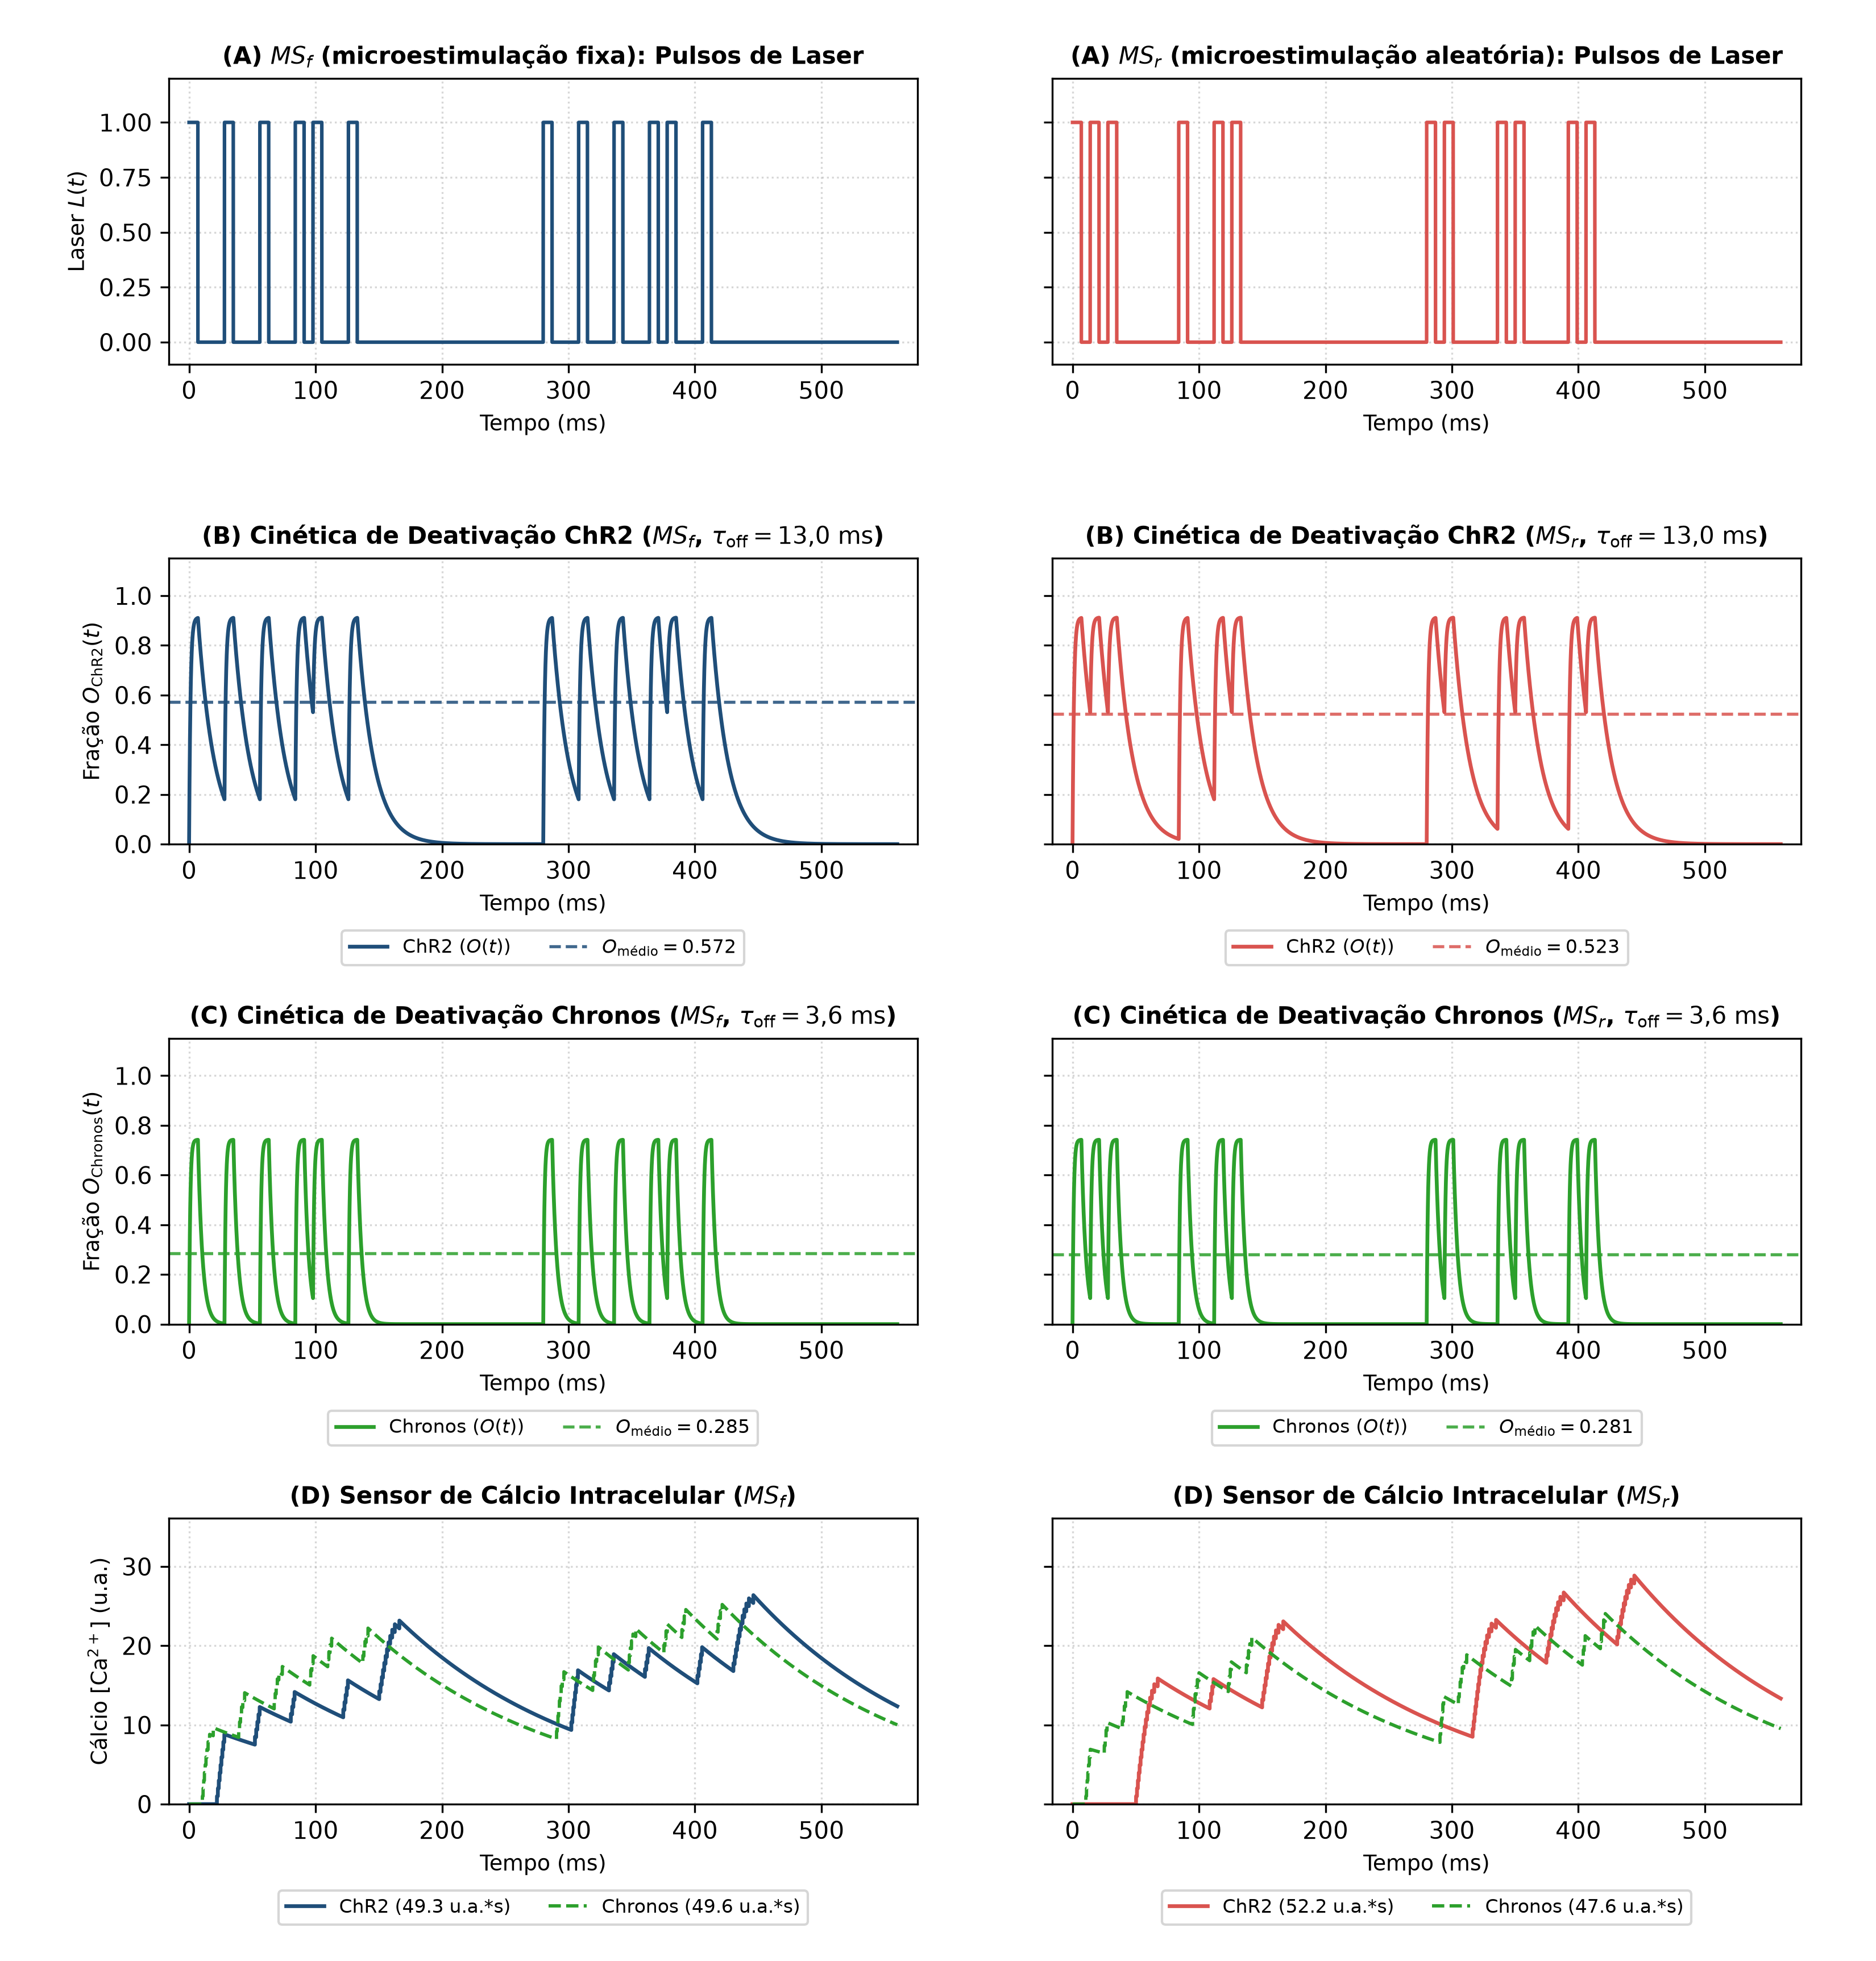
\includegraphics[width=0.95\textwidth,height=0.72\textheight,keepaspectratio]{experimento_2_optogenetica_laura_brian2.png}
    \caption[Simulação em Brian 2 da estimulação optogenética]{Simulação em \textsf{Brian~2} da estimulação optogenética de neurônios piramidais de CA3 com base no protocolo de Costa \cite{costa2026}. Disposição em duas colunas com eixos compartilhados por linha para comparação direta entre a microestimulação fixa ($MS_f$; coluna esquerda) e aleatória ($MS_r$; coluna direita). (A) Trens de pulsos luminosos de laser azul ($\qty{488}{\nano\meter}$, 6 pulsos de $\qty{7}{\milli\second}$ em bins de $\qty{14}{\milli\second}$). (B) Cinética da fração aberta $O(t)$ da opsina clássica ChR2 ($\tau_{\text{off}} = \qty{13{,}0}{\milli\second}$), com a linha tracejada denotando o patamar médio $O_{\text{médio}}$. (C) Cinética da fração aberta $O(t)$ da opsina ultrarrápida Chronos ($\tau_{\text{off}} = \qty{3{,}6}{\milli\second}$) posicionada abaixo de ChR2, com linha tracejada indicando $O_{\text{médio}}$. (D) Dinâmica do sensor de cálcio intracelular $[\text{Ca}^{2+}](t)$, indicador proximal da ativação de c-Fos.}
    \label{fig:exp2_optogenetica}
\end{figure}

\begin{table}[tbp]
    \centering
    \small
    \caption{Cinética fotoquímica e fração de poros abertos $O(t)$ no Experimento 2.}
    \label{tab:resultados_exp2_cinetica}
    \begin{tabular}{llccc}
        \toprule
        \textbf{Opsina} & \textbf{Padrão}    & \textbf{$\tau_{\text{off}}$}                 & \textbf{$O_{\text{médio}}$} & \textbf{$O_{\text{mín}}$} \\
        \midrule
        \multirow{2}{*}{ChR2}
                        & Fixa ($MS_f$)      & \multirow{2}{*}{\qty{13{,}0}{\milli\second}} & $0{,}572$                   & $0{,}180$                 \\
                        & Aleatória ($MS_r$) &                                              & $0{,}548$                   & $0{,}021$                 \\
        \midrule
        \multirow{2}{*}{Chronos}
                        & Fixa ($MS_f$)      & \multirow{2}{*}{\qty{3{,}6}{\milli\second}}  & $0{,}285$                   & $0{,}002$                 \\
                        & Aleatória ($MS_r$) &                                              & $0{,}279$                   & $0{,}000$                 \\
        \bottomrule
    \end{tabular}
    \vspace{0.2em}
    \begin{minipage}{0.95\textwidth}
        \footnotesize \textbf{Nota:} Valores na janela de estimulação ativa ($\qty{140}{\milli\second}$ por ciclo). A ChR2 sustenta patamar residual elevado ($O_{\text{mín}} = 0{,}180$), enquanto a Chronos atinge fechamento completo entre pulsos adjacentes ($O_{\text{mín}} \approx 0$).
    \end{minipage}
\end{table}

\begin{table}[tbp]
    \centering
    \footnotesize
    \setlength{\tabcolsep}{2.2pt}
    \caption{Disparos neuronais, influxo de cálcio intracelular e teste $t$ de Student no Experimento 2.}
    \label{tab:resultados_exp2_calcio}
    \begin{tabular}{llcccc}
        \toprule
        \textbf{Opsina} & \textbf{Padrão}    & \textbf{Disparos/Ciclo} & \textbf{$[\text{Ca}^{2+}]$/Ciclo} & \textbf{Carga Total}                   & \textbf{Teste $t$ ($df=18$)} \\
        \midrule
        \multirow{2}{*}{ChR2}
                        & Fixa ($MS_f$)      & $34{,}10 \pm 0{,}32$    & $4{,}92 \pm 0{,}46$               & \qty{49{,}26}{\text{u.a.}\cdot\second} & $t = -1{,}149$               \\
                        & Aleatória ($MS_r$) & $36{,}10 \pm 2{,}38$    & $5{,}22 \pm 0{,}67$               & \qty{52{,}21}{\text{u.a.}\cdot\second} & $p = 0{,}2656\ (\text{ns})$  \\
        \midrule
        \multirow{2}{*}{Chronos}
                        & Fixa ($MS_f$)      & $34{,}10 \pm 0{,}32$    & $4{,}96 \pm 0{,}37$               & \qty{49{,}62}{\text{u.a.}\cdot\second} & $t = 1{,}116$                \\
                        & Aleatória ($MS_r$) & $32{,}70 \pm 0{,}95$    & $4{,}75 \pm 0{,}45$               & \qty{47{,}56}{\text{u.a.}\cdot\second} & $p = 0{,}2791\ (\text{ns})$  \\
        \bottomrule
    \end{tabular}
    \vspace{0.2em}
    \begin{minipage}{0.95\textwidth}
        \footnotesize \textbf{Nota:} Valores médios $\pm$ desvio padrão sobre $n=10$ ciclos de estimulação ($\qty{280}{\milli\second}$ por ciclo). Unidade de cálcio: $\text{u.a.}\cdot\text{s}$. Teste $t$ de Student bicaudal para amostras independentes sobre a carga de $[\text{Ca}^{2+}](t)$. Ambas as comparações são estatisticamente não significantes ($p > 0{,}05$).
    \end{minipage}
\end{table}


\subsection{Resultados Numéricos e Discussão da Não Diferença Significativa no Estudo Empírico}
Na dissertação experimental de Costa \cite{costa2026}, a quantificação histológica de c-Fos em fatias de CA3 após os protocolos optogenéticos não revelou diferença estatisticamente significante entre os animais submetidos a $MS_f$ e a $MS_r$ ($p = 0{,}9888$), assim como os testes comportamentais de congelamento motor (\emph{freezing}) foram indistinguíveis entre os grupos ($p > 0{,}05$). A análise computacional comparativa e os testes de hipótese inferenciais (\cref{fig:exp2_optogenetica} e \cref{tab:resultados_exp2_cinetica,tab:resultados_exp2_calcio}) fornecem uma base biofísica plausível e formal para esse desfecho empírico:
\begin{enumerate}
    \item \textbf{Efeito de Filtro Passa-Baixas em ChR2:} Com a opsina clássica ChR2 ($\tau_{\text{off}} = \qty{13{,}0}{\milli\second}$), o intervalo de escuridão de $\qty{7}{\milli\second}$ entre pulsos adjacentes é insuficiente para o fechamento espontâneo dos canais (\cref{fig:exp2_optogenetica}B). A fração aberta $O(t)$ não retorna à linha de base, sustentando um patamar residual mínimo elevado ($O_{\text{mín}} = 0{,}180$) e média de $O_{\text{médio}} = 0{,}572$ em $MS_f$ e $0{,}548$ em $MS_r$ (\cref{tab:resultados_exp2_cinetica}). Esse acúmulo atua como um filtro passa-baixas biofísico, convertendo a modulação pulsada em uma despolarização contínua que aplaina as variações temporais. O número de disparos resultou em 341 para $MS_f$ ($\qty{121{,}79}{\hertz}$) e 361 para $MS_r$ ($\qty{128{,}93}{\hertz}$), diferença de $5{,}54\%$. A carga de cálcio intracelular acumulada por ciclo ($\qty{280}{\milli\second}$) foi de $4{,}92 \pm 0{,}46\ \unit{\text{u.a.}\cdot\second}$ para $MS_f$ versus $5{,}22 \pm 0{,}67\ \unit{\text{u.a.}\cdot\second}$ para $MS_r$ ($\Delta = 5{,}66\%$; \cref{tab:resultados_exp2_calcio}). O teste $t$ de Student bicaudal para amostras independentes acusou $t(18) = -1{,}149$, $p = 0{,}2656$ ($p > 0{,}05$, não significante; teste pareado: $t(9) = -1{,}485$, $p = 0{,}1716$), confirmando ausência de separação estatística na carga de cálcio.
    \item \textbf{Resolução Temporal com Chronos versus Invariância de Dose:} Com a cinética rápida de Chronos ($\tau_{\text{off}} = \qty{3{,}6}{\milli\second}$), o canal atinge fechamento praticamente completo durante o escuro ($O_{\text{mín}} = 0{,}002$), restaurando a fidelidade temporal de acompanhamento de cada pulso (\cref{fig:exp2_optogenetica}C). Todavia, como o protocolo experimental fixa rigorosamente a dose total de fótons entregue e o número de pulsos ativos em ambos os padrões (6 pulsos de $\qty{7}{\milli\second}$ por ciclo), a resposta integrada de disparos permaneceu muito próxima: 341 para $MS_f$ ($\qty{121{,}79}{\hertz}$) e 327 para $MS_r$ ($\qty{116{,}79}{\hertz}$), variação de apenas $4{,}11\%$. A carga intracelular de cálcio por ciclo resultou em $4{,}96 \pm 0{,}37\ \unit{\text{u.a.}\cdot\second}$ para $MS_f$ e $4{,}75 \pm 0{,}45\ \unit{\text{u.a.}\cdot\second}$ para $MS_r$ ($\Delta = 4{,}15\%$; \cref{tab:resultados_exp2_calcio}). O teste $t$ de Student independente revelou $t(18) = 1{,}116$, $p = 0{,}2791$ ($p > 0{,}05$, não significante; teste pareado: $t(9) = 1{,}521$, $p = 0{,}1626$).
    \item \textbf{Convergência com a Literatura e Falha Formal em Rejeitar $H_0$:} Ensaios de imunofluorescência quantitativa de c-Fos apresentam dispersão metodológica basal entre $15\%$ e $25\%$, decorrente de variações na permeabilização tecidual e penetração de anticorpos. Como os testes $t$ formais demonstram que as cargas intracelulares de cálcio não apresentam diferença estatisticamente significante ($p = 0{,}2656$ para ChR2 e $p = 0{,}2791$ para Chronos), o poder estatístico do ensaio biológico para detectar separação entre $MS_f$ e $MS_r$ é nulo, convergindo com o valor não significante encontrado na bancada ($p = 0{,}9888$).
    \item \textbf{Por Que Chronos Isolada Não Diferencia e O Que Poderia Viabilizar a Resposta:} Os dados e os testes inferenciais comprovam que a substituição isolada da opsina por uma variante ultrarrápida não basta sob estimulação em malha aberta com dose de fótons casada. Como a cascata de expressão de c-Fos atua como um integrador bioquímico lento na escala de horas, ela é insensível à cronometria microscópica se a carga cumulativa de cálcio for estatisticamente indistinguível ($p > 0{,}25$). Para que padrões temporais alcancem diferenciação funcional real no circuito sob protocolos realizáveis em malha aberta, mecanismos biofísicos não lineares precisam ser recrutados:
          \begin{itemize}
              \item \emph{Modulação por Rajadas de Alta Frequência (Bursting em Malha Aberta):} Concentrar a mesma dose total de fótons em micropulsos de alta frequência ($> \qty{100}{\hertz}$), explorando a não linearidade intrínseca de canais de cálcio dependentes de voltagem de alto limiar (VGCCs tipos L e P/Q) e despolarizações dendríticas locais sustentadas. Em vez de distribuir pulsos uniformemente ao longo do ciclo teta, o agrupamento temporal induz influxo de cálcio supra-aditivo.
              \item \emph{Sintaxe Temporal Calibrada para Janelas de Plasticidade (STDP em Malha Aberta):} Desenhar intervalos inter-pulso (IPIs) calibrados em malha aberta para coincidir com janelas de indução assimétrica de potenciação ($\text{LTP}$, $\Delta t \in [0, +20]\ \unit{\milli\second}$) ou depressão ($\text{LTD}$, $\Delta t \in [-20, 0]\ \unit{\milli\second}$) nas sinapses das colaterais de Schaffer, consolidando a diferenciação temporal em alterações de condutância e conectividade estrutural a longo prazo.
              \item \emph{Multiplexação Óptica Espectral (Dual-Color):} Explorar em modelos computacionais a expressão de opsinas distintas em subpopulações celulares específicas (por exemplo, a opsina excitatória Chronos em neurônios piramidais ativada a $\qty{488}{\nano\meter}$ e a opsina inibitória Chrimson em interneurônios $\text{PV}^+$ ativada a $\qty{625}{\nano\meter}$), permitindo dissociar temporalmente a excitação do freio inibitório perissomático e quebrar a simetria de resposta do microcircuito.
          \end{itemize}
\end{enumerate}

\subsection{Síntese Conclusiva do Experimento 2}
A análise computacional da transdução optogenética sob o protocolo de Costa \cite{costa2026} fundamenta as seguintes conclusões formais:
\begin{enumerate}
    \item \textbf{Decisão Estatística Formal sobre a Hipótese Nula ($H_0$):} \textbf{Não se rejeita $H_0$} em ambas as variantes de opsina:
          \begin{itemize}
              \item \emph{Sob ChR2 Clássica ($\tau_{\text{off}} = \qty{13{,}0}{\milli\second}$):} O teste $t$ de Student independente sobre a carga de cálcio por ciclo resultou em $t(18) = -1{,}149$, $p = 0{,}2656$ ($p > 0{,}05$, não significante; $\Delta_{\text{Cálcio}} = 5{,}66\%$; \cref{tab:resultados_exp2_calcio}).
              \item \emph{Sob Chronos Rápida ($\tau_{\text{off}} = \qty{3{,}6}{\milli\second}$):} Apesar de a opsina rápida fechar completamente entre pulsos adjacentes ($O_{\text{mín}} \approx 0$; \cref{tab:resultados_exp2_cinetica}), o teste $t$ de Student resultou em $t(18) = 1{,}116$, $p = 0{,}2791$ ($p > 0{,}05$, não significante; $\Delta_{\text{Cálcio}} = 4{,}15\%$).
          \end{itemize}
          Ambas as comparações são estatisticamente não significantes ($p > 0{,}25$), situando-se expressivamente abaixo da dispersão biológica basal típica de imunofluorescência de c-Fos ($15\%\text{ a }25\%$), comprovando matematicamente por que os dois padrões são indistinguíveis sob essa via molecular.
    \item \textbf{Convergência com os Dados Empíricos de Bancada:} A modelagem biofísica associada aos testes inferenciais oferece a justificativa quantitativa rigorosa para a ausência de significância estatística reportada por Costa \cite{costa2026} tanto na densidade celular de c-Fos em fatias histológicas de CA3 ($p = 0{,}9888$) quanto nos escores comportamentais de congelamento motor (\emph{freezing}, $p > 0{,}05$) entre os animais dos grupos $MS_f$ e $MS_r$.
    \item \textbf{Limitações da Malha Aberta e Conclusão Biofísica:} O modelo demonstra que acelerar a cinética do canal através de uma opsina ultrarrápida é condição necessária, mas insuficiente, para quebrar a simetria funcional do tecido quando o protocolo opera em malha aberta com dose de fótons estritamente pareada (mesmo número e largura de pulsos). Como a via de c-Fos atua como um integrador lento de carga, a diferenciação biológica real sob regimes de malha aberta exige o recrutamento de mecanismos não lineares que interajam com a dinâmica interna da rede (modulação temporal por rajadas em alta frequência para recrutamento supralinear de VGCCs, sintaxe temporal calibrada para janelas assimétricas de STDP ou multiplexação espectral de tipos celulares).
\end{enumerate}

\chapter[Proposta de Continuação do Mestrado]{Proposta de Continuação do Mestrado}

A análise crítica dos dados comportamentais existentes, combinada com os resultados de simulação biofísica em \textsf{Brian~2}, delimita o escopo de continuidade para o mestrado no PPGEE/UFMG. Em consonância com a trajetória acadêmica e profissional na Engenharia Elétrica e respeitando os limites dos dados já coletados, a etapa experimental com animais encontra-se \textbf{concluída}, não havendo previsão de novas manipulações cirúrgicas ou testes de biotério.

O plano de trabalho proposto concentra-se inteiramente no tratamento analítico dos dados disponíveis e na expansão da modelagem computacional teórica (\emph{in silico}) em regimes de malha aberta:

\begin{enumerate}
    \item \textbf{Consolidação Metrológica dos Dados Comportamentais de Bancada:} Finalizar a sistematização e a análise inferencial descritiva dos lotes experimentais já executados (\#1 a \#6), formalizando a documentação sobre controle de viés físico em testes de preferência e quantificando o impacto do subdimensionamento amostral sobre o poder estatístico em estudos de roedores.
    \item \textbf{Modelagem de Plasticidade Sináptica (STDP) no Eixo CA3--CA1:} Expandir os microcircuitos em \textsf{Brian~2} para modelar a transmissão de sinais através das colaterais de Schaffer, incorporando regras biofísicas de plasticidade sináptica dependente do tempo de disparo (\emph{Spike-Timing-Dependent Plasticity} -- STDP). O objetivo é avaliar teoricamente como padrões temporais discretizados em malha aberta com diferentes intervalos inter-pulso (IPIs) modulam a potenciação ($\text{LTP}$) ou depressão ($\text{LTD}$) sináptica a longo prazo.
    \item \textbf{Simulação Computacional de Protocolos em Malha Aberta Baseados em Rajadas (\emph{Bursting}):} Investigar computacionalmente o impacto de protocolos de estimulação óptica baseados em rajadas breves de alta frequência ($> \qty{100}{\hertz}$) em malha aberta versus pulsos uniformemente espaçados sob mesma densidade de energia luminosa (dose idêntica de fótons), quantificando a indução cooperativa de influxo de cálcio dendrítico via VGCCs e a dinâmica de recuperação vesicular sináptica.
    \item \textbf{Modelagem Computacional de Multiplexação Óptica Espectral:} Simular o recrutamento diferencial de populações celulares por meio de duas opsinas espectralmente distintas (ativação excitatória rápida via Chronos em $\qty{488}{\nano\meter}$ e inibitória seletiva via Chrimson em $\qty{625}{\nano\meter}$), investigando como o desacoplamento temporal entre excitação e inibição pode gerar estados funcionais discrimináveis em redes recorrentes em malha aberta.
\end{enumerate}

\newpage

% --- Apêndices ---
\begin{apendicesenv}

    \chapter{Fundamentação Didática dos Mecanismos Neurofisiológicos Modelados}
    \label[appendix]{apendice:mecanismos_neurofisiologicos}

    Este apêndice compila as bases biológicas e biofísicas dos componentes celulares e sinápticos representados nas simulações computacionais em \textsf{Brian~2}. Sua finalidade primordial é servir como material de estudo e consolidação conceitual para o autor, estruturando formalmente a interface entre o processamento de sinais em engenharia e a neurofisiologia de circuitos excitáveis, sem truncar o fluxo dos capítulos principais para pesquisadores e docentes da área médica ou biológica.

    O processamento e a propagação de perturbações artificiais --- sejam campos elétricos extracelulares ou pulsos luminosos de laser absorvidos por canais de opsinas --- decorrem da interação coordenada de cinco subsistemas celulares e moleculares interdependentes \cite{buzsaki2006, kandel2021}:

    \section{Neurônios Piramidais Excitatórios (Regular Spiking -- RS)}
    Representam as unidades principais de integração e projeção glutamatérgica da região CA3 do hipocampo \cite{kandel2021}. Possuem corpos celulares piramidais e uma extensa árvore dendrítica que recebe aferências do giro denteado (fibras musgosas), do córtex entorrinal (via perfurante) e de células piramidais vizinhas (colaterais recorrentes). Eletrofisiologicamente, comportam-se como integradores com adaptação lenta de frequência de disparo (\emph{Regular Spiking}): sob injeção constante de corrente despolarizante, respondem inicialmente com alta taxa de disparo, que decai exponencialmente para uma frequência estacionária moderada \cite{dayan2001, gerstner2014}. Essa adaptação é mediada pelo acúmulo gradual de condutâncias de potássio ativadas por voltagem e por cálcio intracelular ($I_M$, $I_{\text{AHP}}$), exercendo retroalimentação hiperpolarizante contínua \cite{izhikevich2007}.

    \section{Interneurônios Inibitórios Locais \texorpdfstring{$\text{PV}^+$}{PV+} (Fast Spiking -- FS)}
    Constituem a principal população de interneurônios inibitórios GABAérgicos perissomáticos, caracterizados pela expressão citoplasmática da proteína ligadora de cálcio parvalbumina ($\text{PV}$) \cite{buzsaki2006, kandel2021}. No microcircuito, atuam como controladores rápidos de ganho dinâmico e sincronizadores de rede. Em virtude de sua menor capacitância transmembrana, canais de potássio ultra-rápidos do tipo Kv3 e baixa reobase, disparam potenciais de ação com menor injeção de corrente do que células piramidais e sustentam frequências elevadas ($> \qty{150}{\hertz}$) sem sofrer adaptação \cite{izhikevich2003, izhikevich2007}. Essa propriedade confere a essas células a capacidade de impor janelas temporais de inibição extremamente estreitas e inflexíveis sobre os neurônios principais.

    \section{Inibição Perissomática por Shunting}
    Os interneurônios $\text{PV}^+$ direcionam seus terminais axônicos especificamente ao soma e ao segmento inicial do axônio das células piramidais, liberando o neurotransmissor inibitório GABA \cite{buzsaki2006, kandel2021}. O GABA liga-se a receptores ionotrópicos pós-sinápticos $\text{GABA}_A$, promovendo a abertura de condutâncias permeáveis ao íon cloreto ($\text{Cl}^-$). Como o potencial de reversão do cloreto ($E_{\text{GABA}} \approx \qty{-75}{\milli\volt}$) situa-se muito próximo do potencial de repouso fisiológico da célula ($\approx \qty{-65}{\milli\volt}$), a ativação desses canais acarreta pouca deflexão hiperpolarizante líquida de voltagem, mas provoca uma drástica elevação na condutância de membrana \cite{dayan2001, gerstner2014}. No domínio da teoria de circuitos elétricos, esse mecanismo equivale à inserção de uma condutância elevada (resistor de baixo valor ôhmico) em paralelo com a membrana para a referência de terra (\emph{shunting inhibition}). Quaisquer correntes despolarizantes incidentes (oriundas de microeletrodos extracelulares ou excitação sináptica) são drenadas preferencialmente através dessa via de baixa impedância antes que a capacitância celular seja carregada até o limiar de disparo.

    \section{Depressão Sináptica de Curto Prazo (Short-Term Depression -- STD)}
    A transmissão de sinais químicos através de junções sinápticas exibe dinâmica não-linear variante no tempo \cite{dayan2001, gerstner2014}. No botão pré-sináptico, os neurotransmissores concentram-se em vesículas armazenadas no chamado reservatório prontamente liberável (\emph{Readily Releasable Pool} -- RRP) \cite{kandel2021}. A cada potencial de ação invasor, uma fração finita $U$ desse reservatório é liberada por exocitose na fenda sináptica. O processo biofísico de reciclagem, docagem, ancoragem e priming de novas vesículas é bioquimicamente lento, sendo modelado por uma constante de recuperação $\tau_{\text{rec}} \approx \qty{600}{\milli\second}$ \cite{tsodyks1997, tsodyks1998}. Sob trens de pulsos repetitivos com intervalos inter-pulso (IPIs) muito menores do que $\tau_{\text{rec}}$ (como em frequências de $\qty{10}{\hertz}$ a $\qty{70}{\hertz}$), o reservatório vesicular esgota-se rapidamente, colapsando a amplitude dos potenciais pós-sinápticos subsequentes para um nível basal deprimido.

    \section{Fotoestimulação e Cinética Biofísica de Opsinas Microbianas}
    Na tecnologia optogenética, canais iônicos sensíveis à luz derivados de algas ou microrganismos são direcionados geneticamente para populações neuronais específicas \cite{boyden2005, deisseroth2011}. Ao absorverem fótons em comprimentos de onda de ressonância (ex.: $\qty{488}{\nano\meter}$ para ChR2), as moléculas de retinal isomerizam-se, comutando o poro para uma conformação aberta condutiva para cátions ($\text{Na}^+$, $\text{Ca}^{2+}$) \cite{nagel2003}. O retorno ao estado inativo fechado ao cessar a iluminação não é instantâneo, dependendo de relaxamento térmico fotoquímico governado por uma constante de desativação $\tau_{\text{off}}$ \cite{nikolic2009, grossman2011}. Para variantes clássicas como a ChR2 nativa ($\tau_{\text{off}} \approx \qty{13}{\milli\second}$), intervalos escuros inferiores a essa constante impedem o fechamento do canal, fundindo pulsos ópticos discretos em uma onda contínua de influxo iônico (comportamento de filtro passa-baixas). Opsinas de engenharia molecular com cinética acelerada, como a Chronos ($\tau_{\text{off}} \approx \qty{3{,}6}{\milli\second}$), possibilitam que o poro feche rapidamente entre pulsos subsequentes, restaurando a fidelidade temporal de disparo \cite{klapoetke2014}.

\end{apendicesenv}

% --- Elementos Pós-Textuais ---
\postextual

\bibliography{referencias}

\end{document}